\section{系统测试}

\subsection{注册登录功能测试}

% 系统测试是针对整个产品系统进行的测试,目的是验证系统是否满足了需求规格的定义,找出与需求规格不符或与之矛盾的地方,从而提出更加完善的方案。系统测试发现问题之后要经过调试找出错误原因和位置,然后进行改正,是基于系统整体需求说明书的黑盒类测试,应覆盖系统所有联合的部件。

进入到智慧工厂管理系统之后,在上方导航栏处有登陆按钮,点击之后即可输入账号名与密码进行登录,对于初次使用本系统的工厂管理人员,在登录界面有方有注册按钮,即可对当前部门组织进行注册。如表\ref{tab:rgstlgfuct}所示注册登录功能的用例表。

\begin{table}[H]
    \zihao{5}
    \centering
    \caption{注册登录功能用例表}
    \label{tab:rgstlgfuct}
    \begin{tabularx}{.95\textwidth}{X<{\centering}X<{\centering}p{16em}<{\centering}X<{\centering}X<{\centering}}
        \toprule
        序号 & 操作 & 输入及说明 & 期望结果 & 实际结果 \\
        \midrule
        1 & 注册 & 按照系统提示输入正确的注册信息 & 注册成功 & 预期结果 \\
        2 & 注册 & 用户名输入框内输入重复信息注册 & 注册失败 & 预期结果 \\
        3 & 注册 & 在输入框内输入特殊字符 & 注册失败 & 预期结果 \\
        4 & 登录 & 按照系统提示输入正确的登录信息 & 登录成功 & 预期结果 \\
        5 & 注册 & 输入错误的账号名或密码 & 登录失败 & 预期结果 \\
        \bottomrule
    \end{tabularx}
\end{table}

注册时填入注册所需提供的信息之后点击注册按钮,若注册信息填写有误,例如用户名已经被使用,则在上方发出错误信息提示,如图\ref{fig:rgster}所示。

\begin{figure}[H]
    \centering
    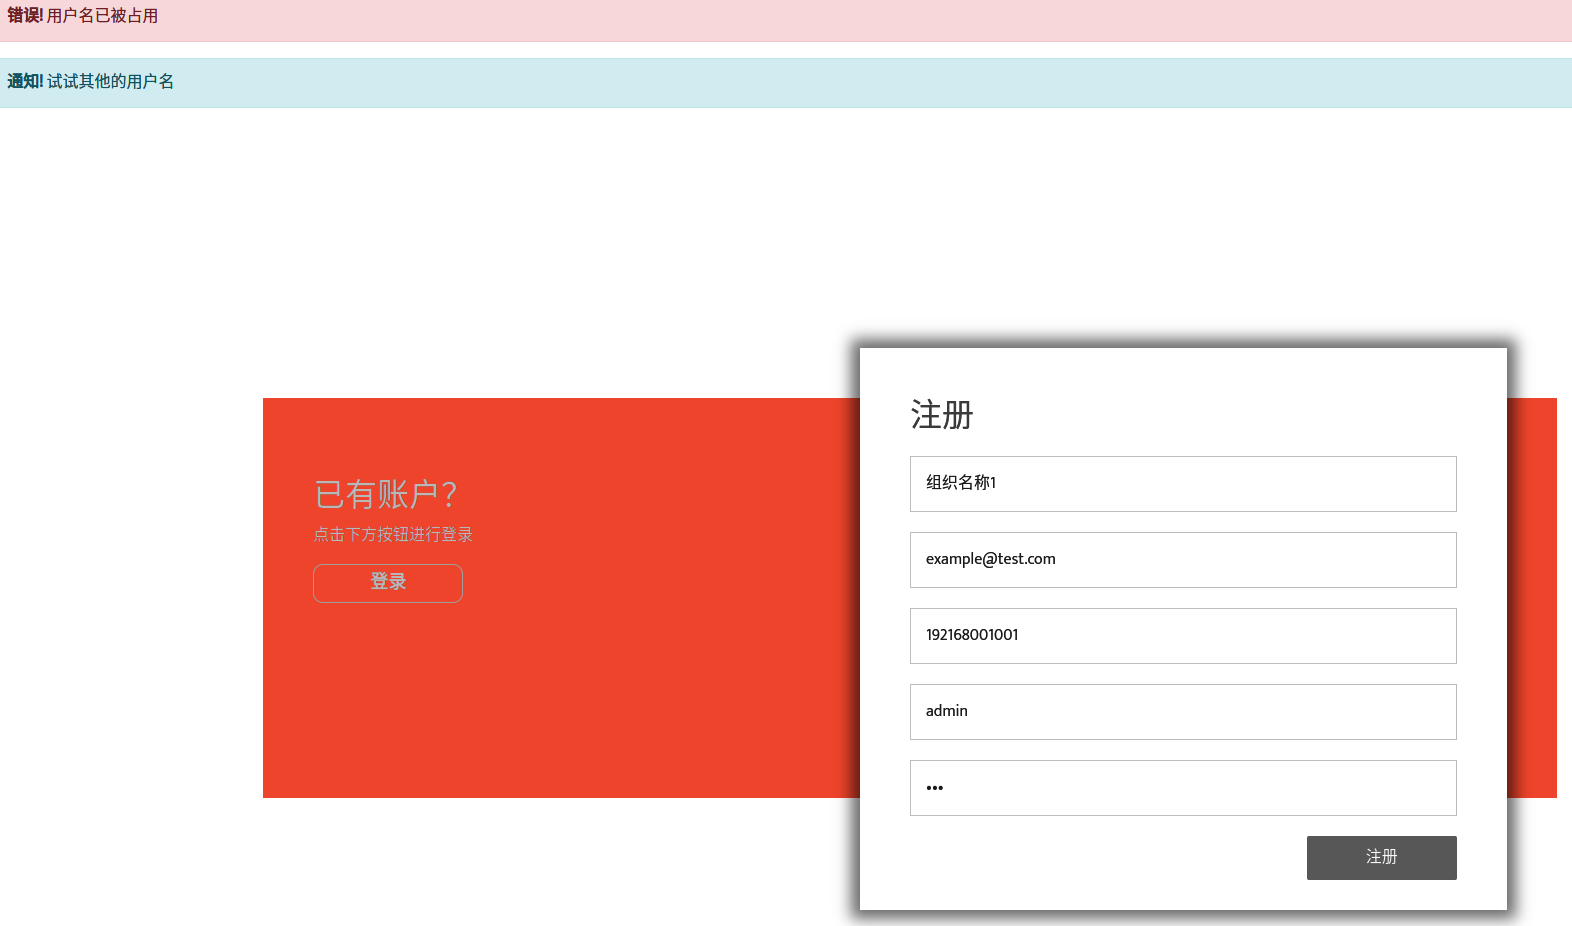
\includegraphics[width=.45\textwidth]{figures/6registererror.png}
    \caption{注册信息填入错误提示图}
    \label{fig:rgster}
\end{figure}

注册成功之后,在登录界面输入账户名与密码进行登录,登录成功之后,进入后台管理页面并且在上方显示欢迎用户的消息提示,如图\ref{fig:lgsccs}所示。

\begin{figure}[H]
    \centering
    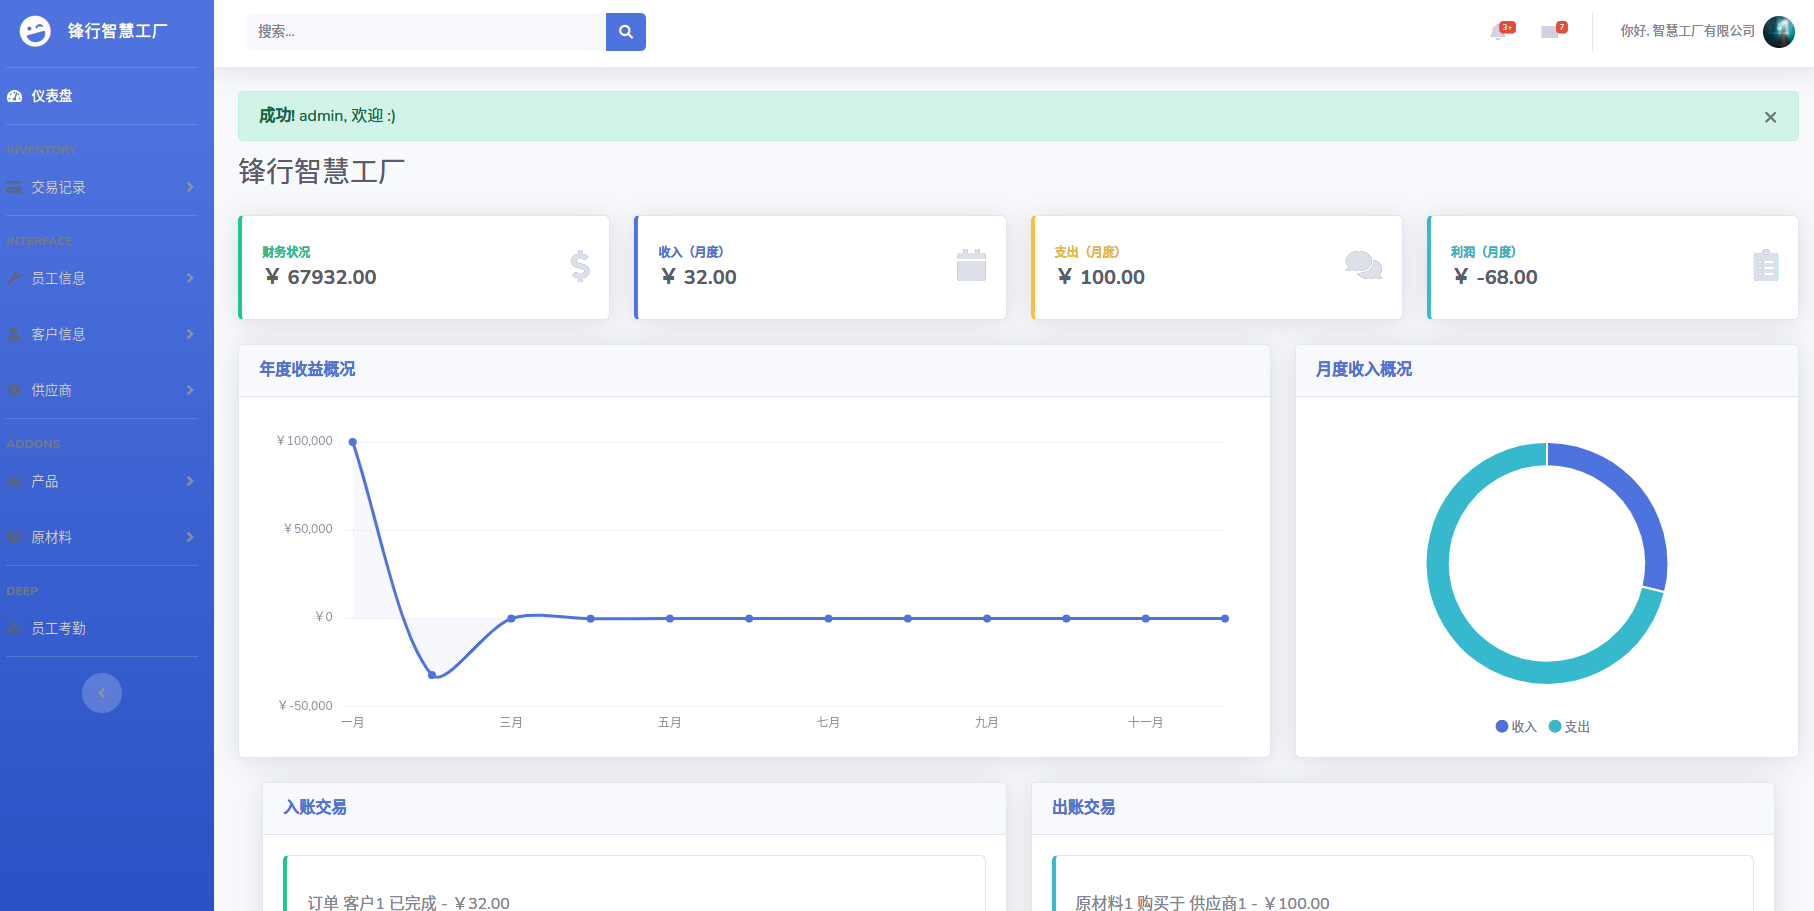
\includegraphics[width=.65\textwidth]{figures/6loginsuscess.png}
    \caption{登录成功消息提示图}
    \label{fig:lgsccs}
\end{figure}

\subsection{工厂信息管理功能测试}

进入后台管理页面之后,可以对当前工厂部门组织的信息进行管理,其中包括交易记录管理、员工信息管理、客户信息管理、供应商信息管理、产品信息管理以及原材料信息管理等。表\ref{tab:ifmtmngmt}为工厂信息管理功能的测试用例表。在单元上执行集成测试后,这些单元将组合到各个模块中,然后必须将其作为一个完整的系统进行系统测试。

\begin{table}[H]
    \zihao{5}
    \centering
    \caption{信息管理功能用例表}
    \label{tab:ifmtmngmt}
    \begin{tabularx}{.95\textwidth}{p{2em}<{\centering}X<{\centering}p{16em}<{\centering}X<{\centering}X<{\centering}}
        \toprule
        序号 & 操作 & 输入及说明 & 期望结果 & 实际结果 \\
        \midrule
        1 & 添加员工 & 按照系统提示输入正确的员工信息 & 添加成功 & 预期结果 \\
        2 & 编辑员工 & 根据系统提示输入更新的员工信息 & 更新成功 & 预期结果 \\
        3 & 添加任务 & 指定员工添加工作任务 & 添加成功 & 预期结果 \\
        4 & 添加任务 & 输入大于原材料数量的产能 & 添加失败 & 预期结果 \\
        5 & 添加产品 & 根据系统提示输入正确的产品信息 & 添加成功 & 预期结果 \\
        6 & 支付薪资 & 指定员工支付当前月薪 & 支付成功 & 预期结果 \\
        7 & 支付薪资 & 账户余额不足的情况下支付薪资 & 支付失败 & 预期结果 \\
        8 & 添加客户 & 按照系统提示输入正确的客户信息 & 添加成功 & 预期结果 \\
        9 & 产品下单 & 指定客户对产品进行下单 & 下单成功 & 预期结果 \\
        10 & 产品下单 & 当前部门产品数量不足的下单操作 & 下单失败 & 预期结果 \\
        10 & 产品派送 & 指定订单进行派送操作 & 派送成功 & 预期结果 \\
        11 & 产品派送 & 产品数量不足进行派送操作 & 派送失败 & 预期结果 \\
        12 & 添加供应商 & 按照系统提示输入正确的供应商信息 & 添加成功 & 预期结果 \\
        13 & 原材料采购 & 指定供应商对原材料类型进行采购 & 采购成功 & 预期结果 \\
        14 & 原材料采购 & 账户余额不足的情况下采购操作 & 采购失败 & 预期结果 \\
        \bottomrule
    \end{tabularx}
\end{table}

如图\ref{fig:tscttf}所示为交易记录的信息管理图。左图为查看所有交易记录详情,右图为添加交易记录页面。

\begin{figure}[H]
    \centering
    \begin{subfigure}{.45\textwidth}
        \centering
        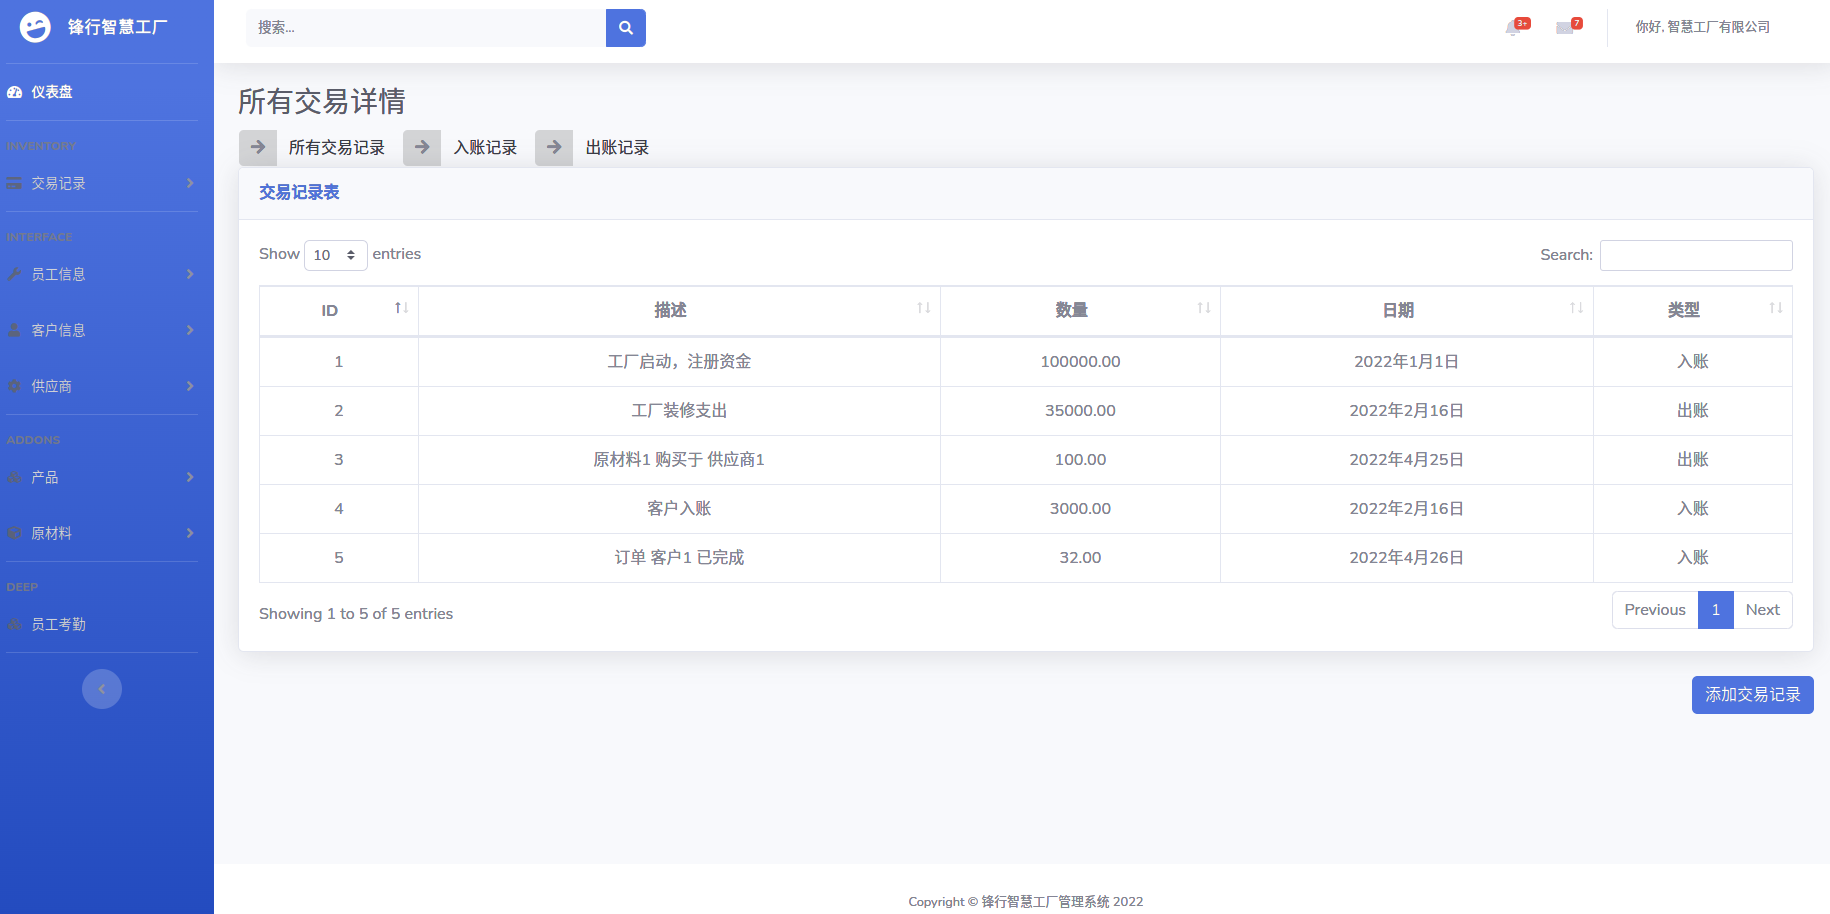
\includegraphics[width=\textwidth]{figures/6viewalltransc.png}
        % \subcaption{查看交易记录详情图}
        % \label{fig:vuatsc}
    \end{subfigure}
    \qquad
    \begin{subfigure}{.45\textwidth}
        \centering
        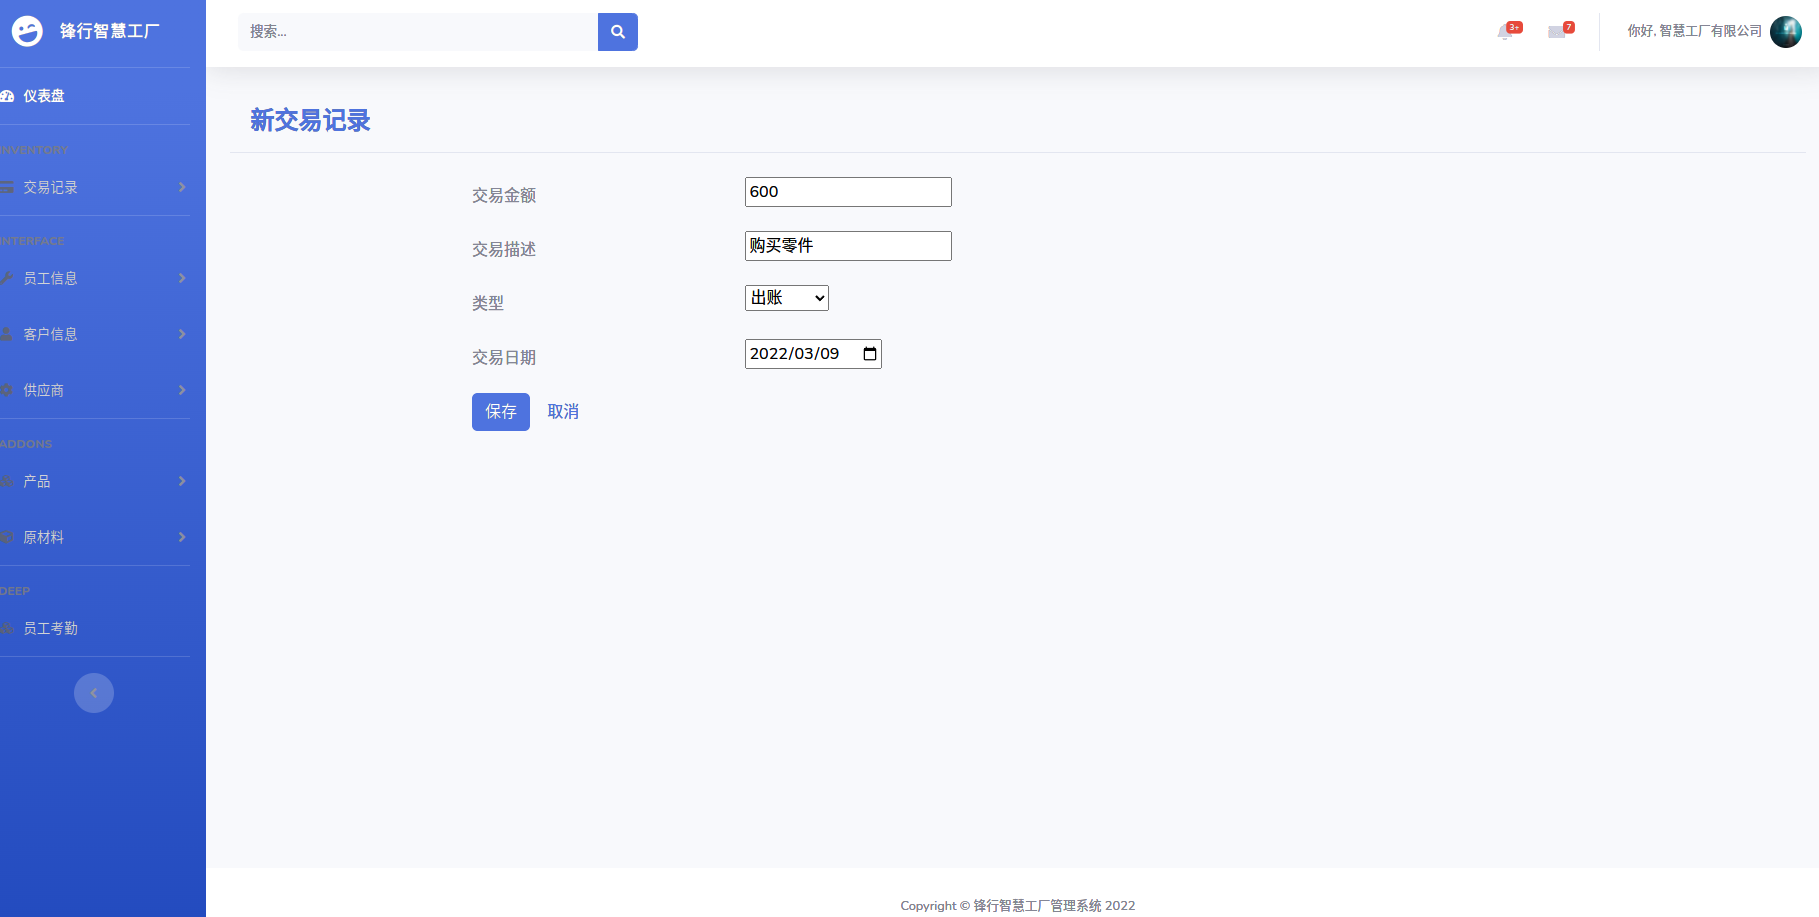
\includegraphics[width=\textwidth]{figures/6addnewtransc.png}
        % \subcaption{添加交易记录测试图}
        % \label{fig:adnutsc}
    \end{subfigure}
    \caption{交易记录信息管理测试图}
    \label{fig:tscttf}
\end{figure}

关于员工信息管理,包括查看员工、添加员工、支付薪资以及下单工作任务等功能,如图\ref{fig:emploetest}所示。其中包括查看所有员工信息详情、为添加员工页面功能测试、为员工支付当前月薪功能测试以及为指定员工指派工作任务功能测试。

\begin{figure}[H]
    % \centering
    % \begin{subfigure}{.45\textwidth}
        \centering
        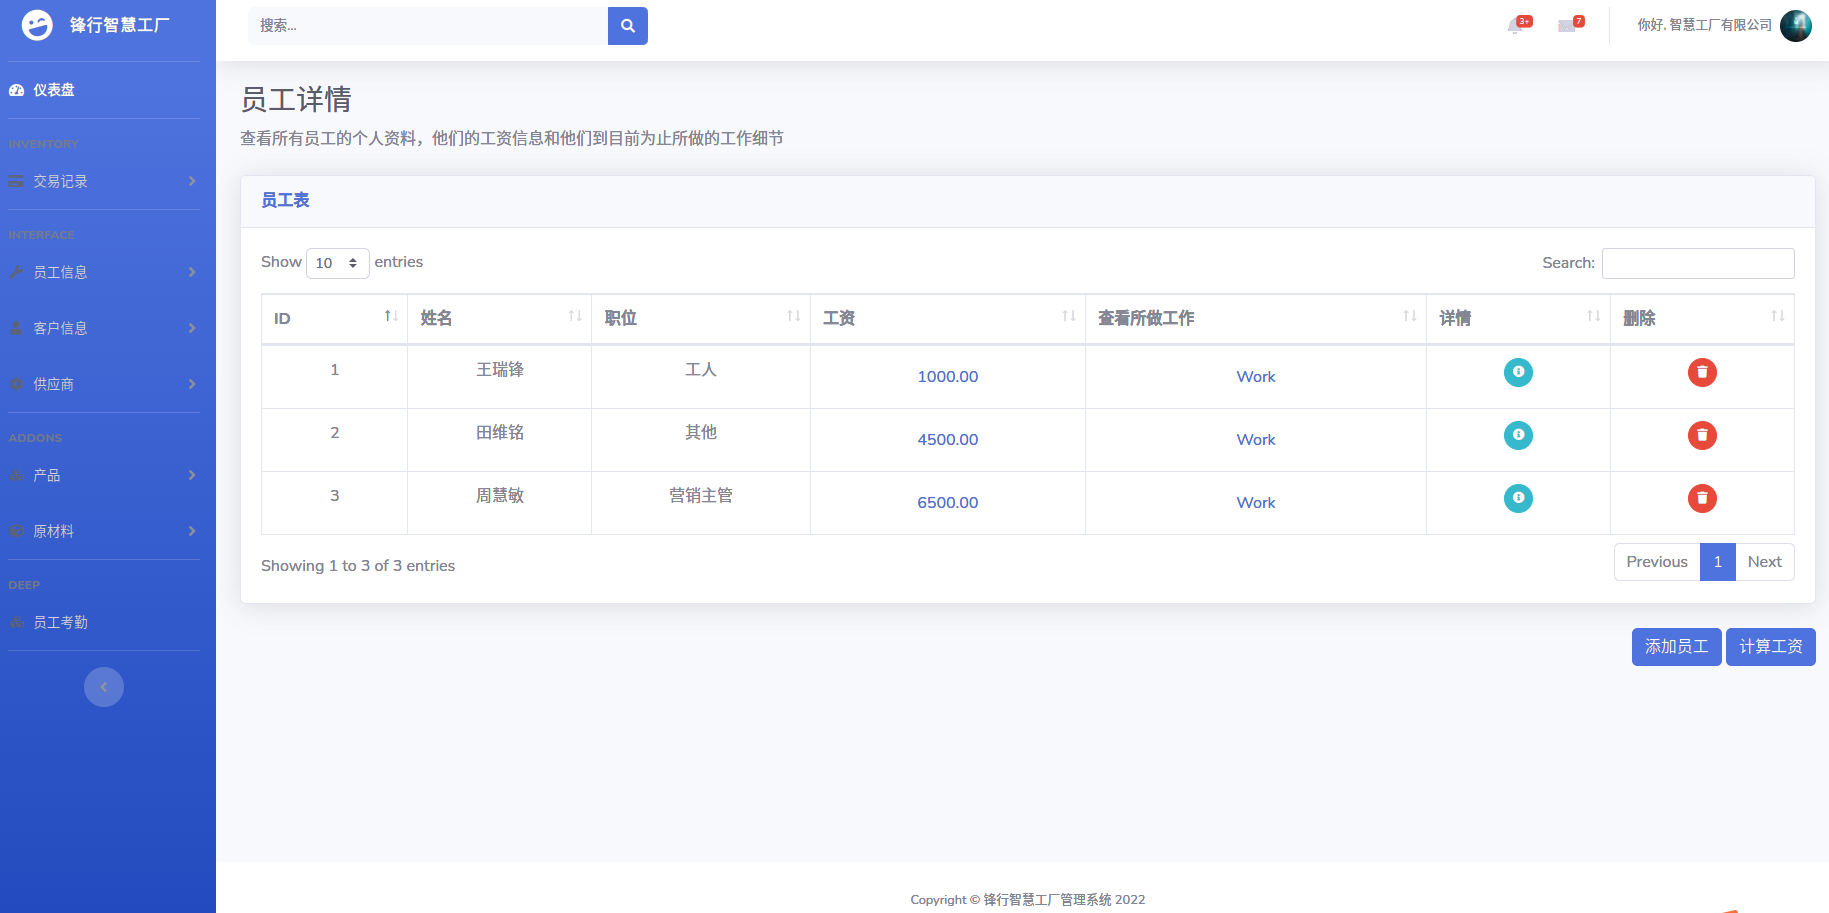
\includegraphics[width=.75\textwidth]{figures/6viewallemployee.png}
        % \subcaption{查看员工信息详情图}
        % \label{fig:vuaemple}
    % \end{subfigure}
    % \qquad
    % \begin{subfigure}{.45\textwidth}
    %     \centering
    %     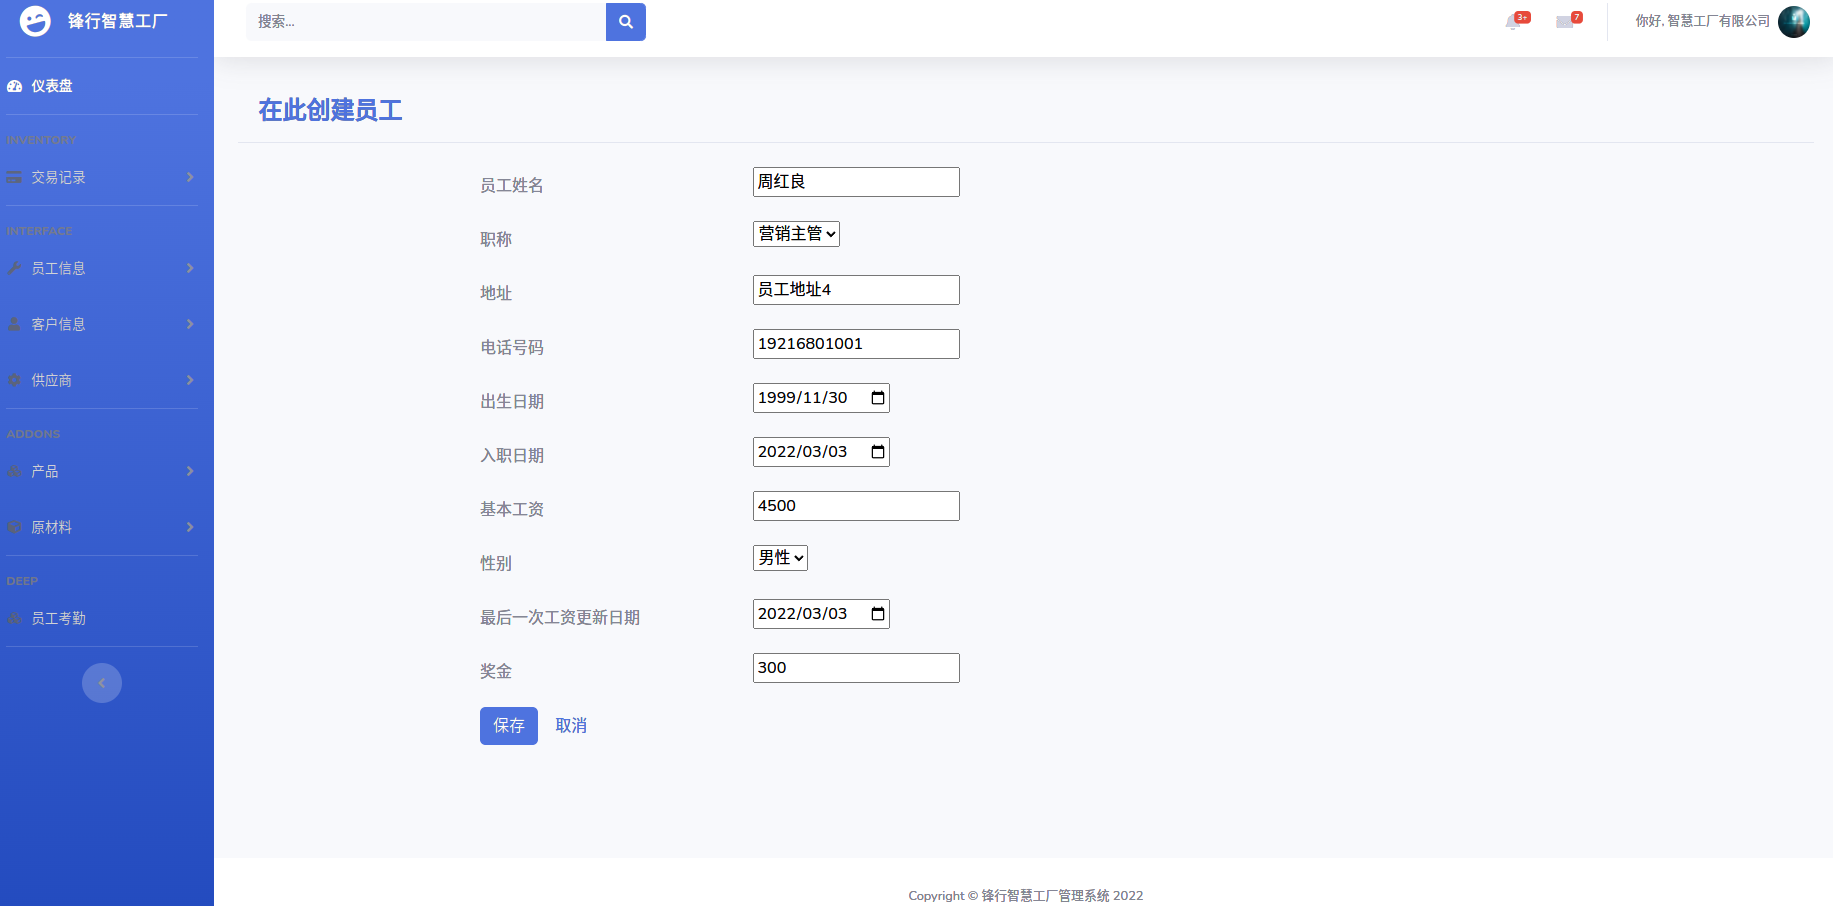
\includegraphics[width=\textwidth]{figures/6addnewemployee.png}
    %     % \subcaption{添加员工测试图}
    %     % \label{fig:adnuemploe}
    % \end{subfigure}
    % \\
    % \begin{subfigure}{.45\textwidth}
    %     \centering
    %     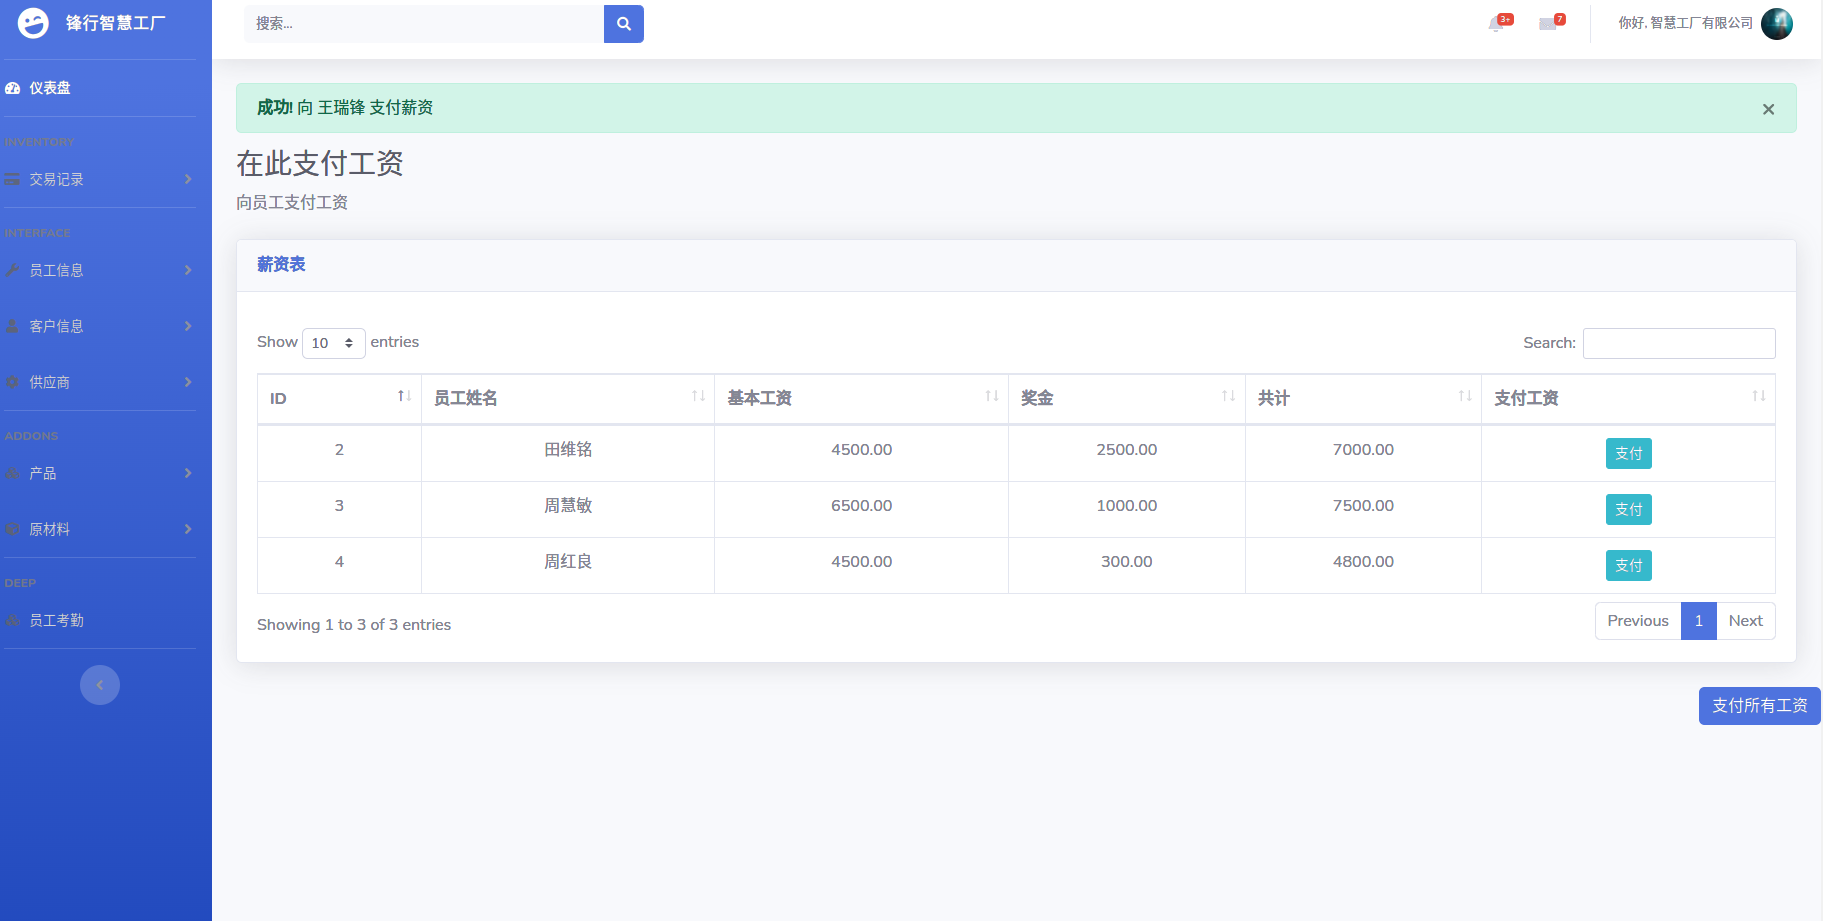
\includegraphics[width=\textwidth]{figures/6paysalary.png}
    %     % \subcaption{向员工支付薪资测试图}
    %     % \label{fig:pyslr}
    % \end{subfigure}
    % \qquad
    % \begin{subfigure}{.45\textwidth}
    %     \centering
    %     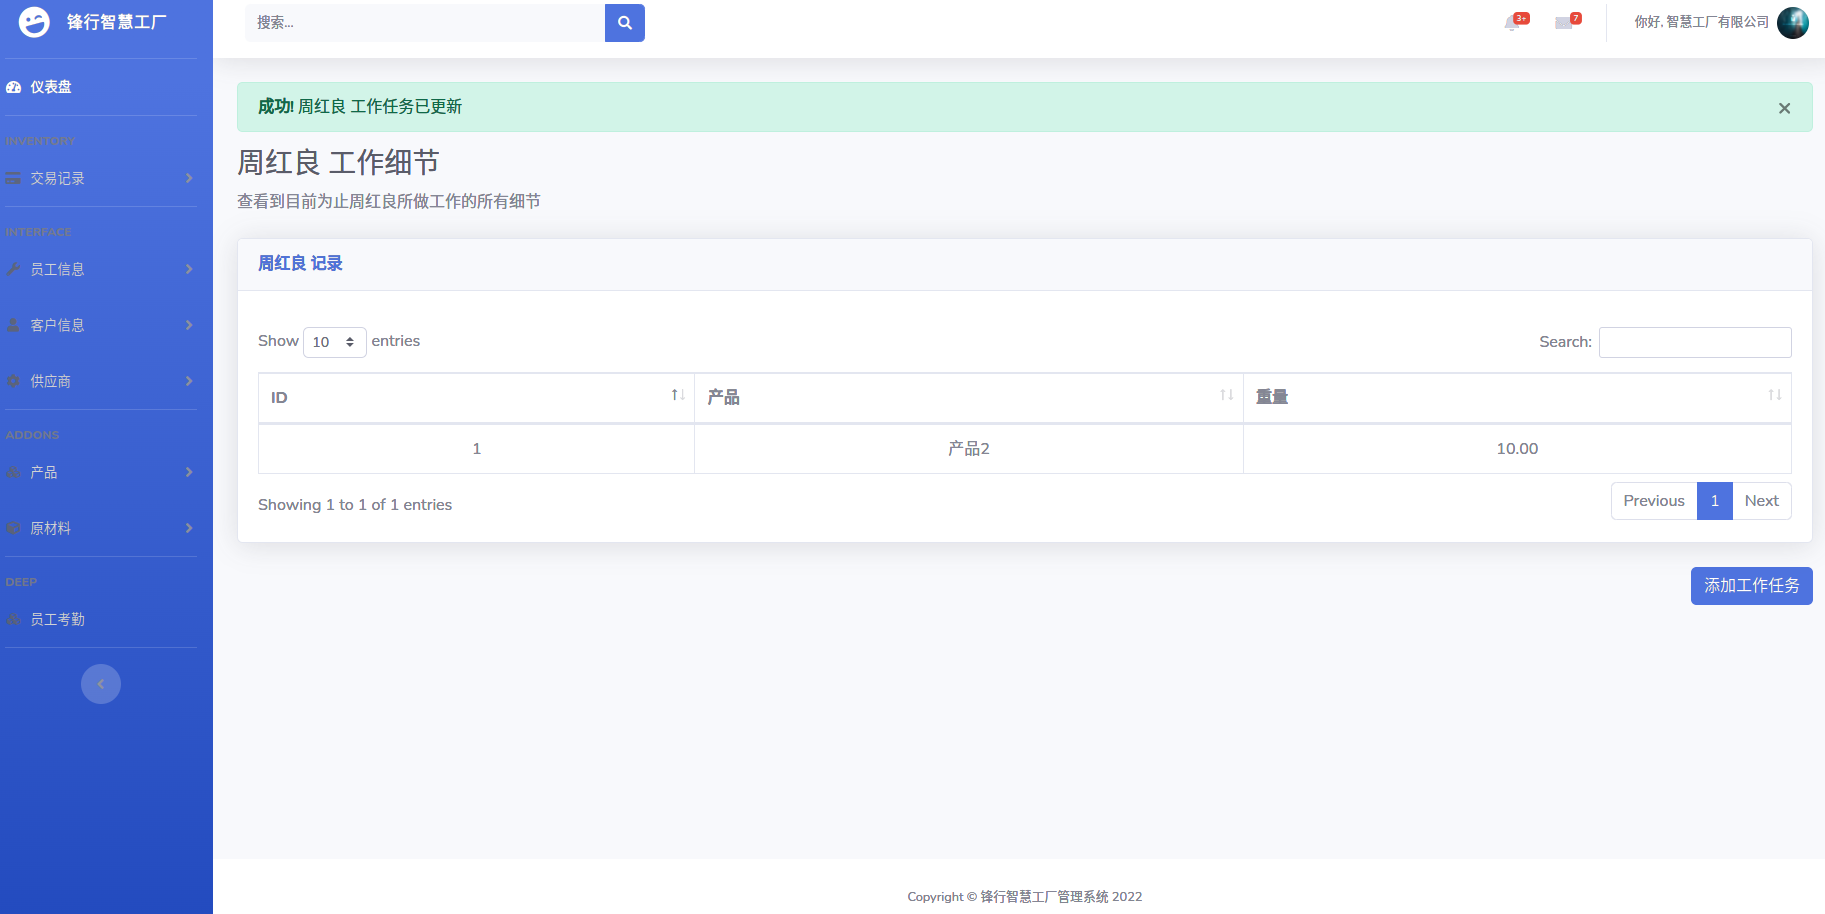
\includegraphics[width=\textwidth]{figures/6addwork.png}
    %     % \subcaption{添加员工工作任务测试图}
    %     % \label{fig:addwork}
    % \end{subfigure}
    \caption{员工信息管理测试图}
    \label{fig:emploetest}
\end{figure}

客户信息管理包括查看所有客户信息详情、添加客户信息、为指定客户下单、查看客户信息订单以及订单详细收据等功能,如图\ref{fig:cstmtst}所示。其中包括查看所有客户信息详情功能测试图、为添加客户信息功能测试、为查看所有客户订单的功能测试以及查看指定订单收据功能测试。

\begin{figure}[H]
    \centering
    \begin{subfigure}{.45\textwidth}
        \centering
        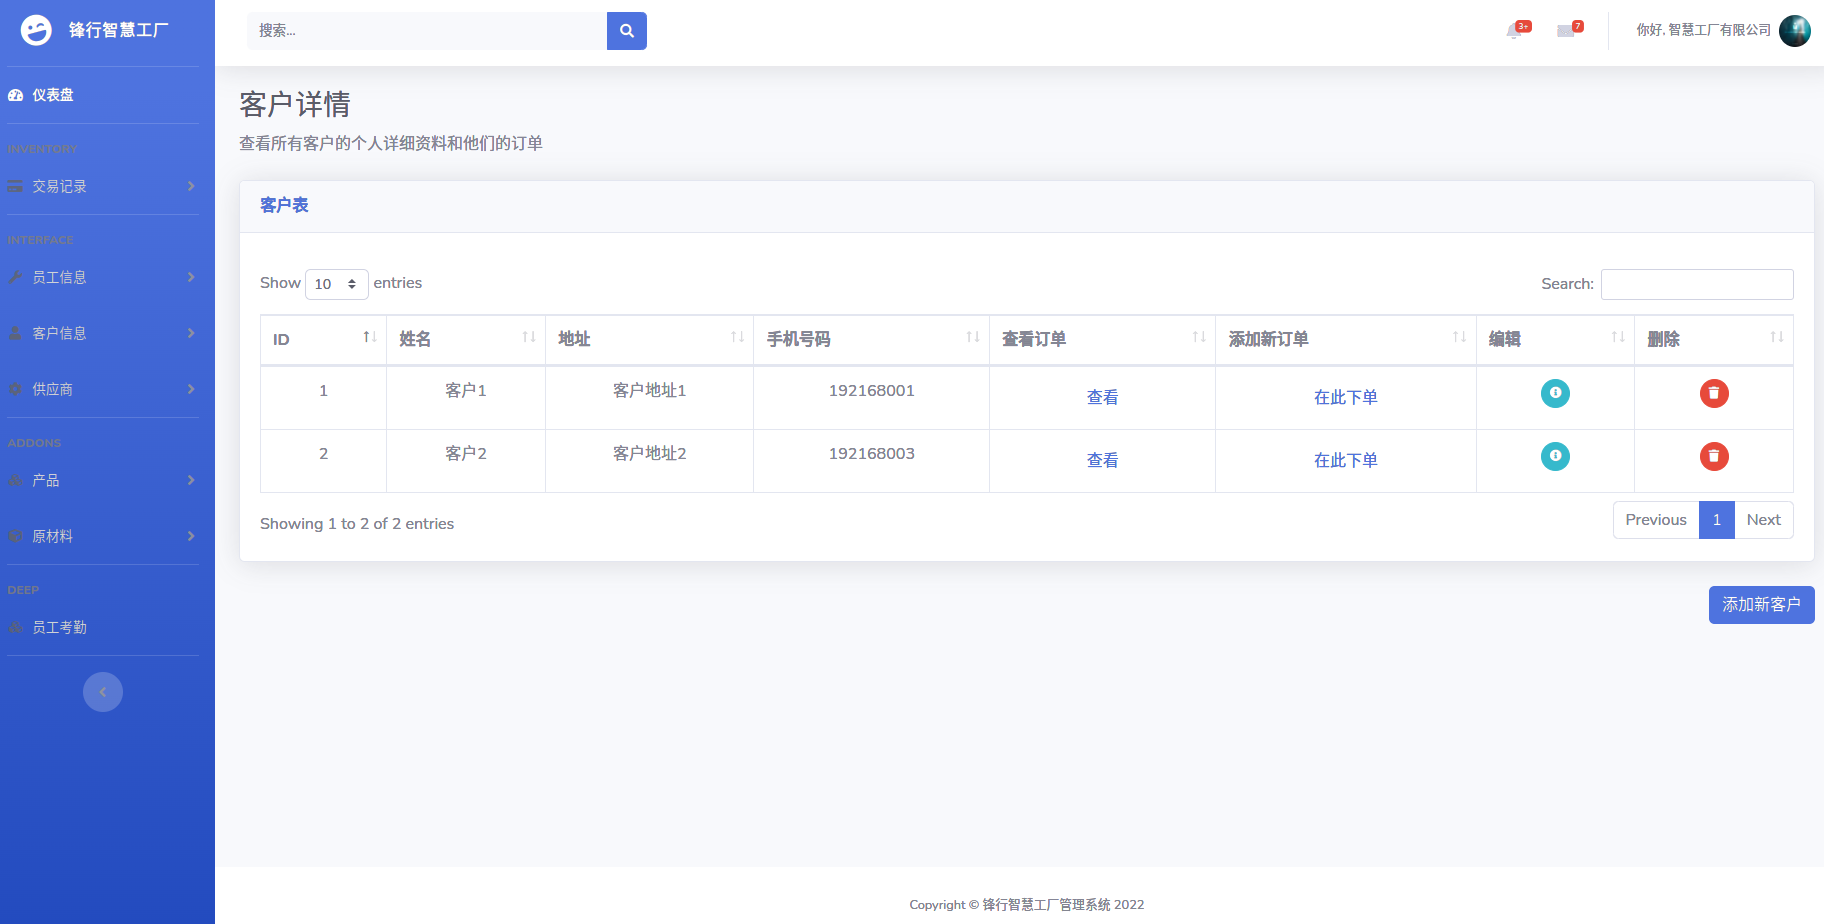
\includegraphics[width=\textwidth]{figures/6viewallcustomer.png}
        % \subcaption{查看客户信息详情图}
        % \label{fig:vuacstm}
    \end{subfigure}
    \qquad
    \begin{subfigure}{.45\textwidth}
        \centering
        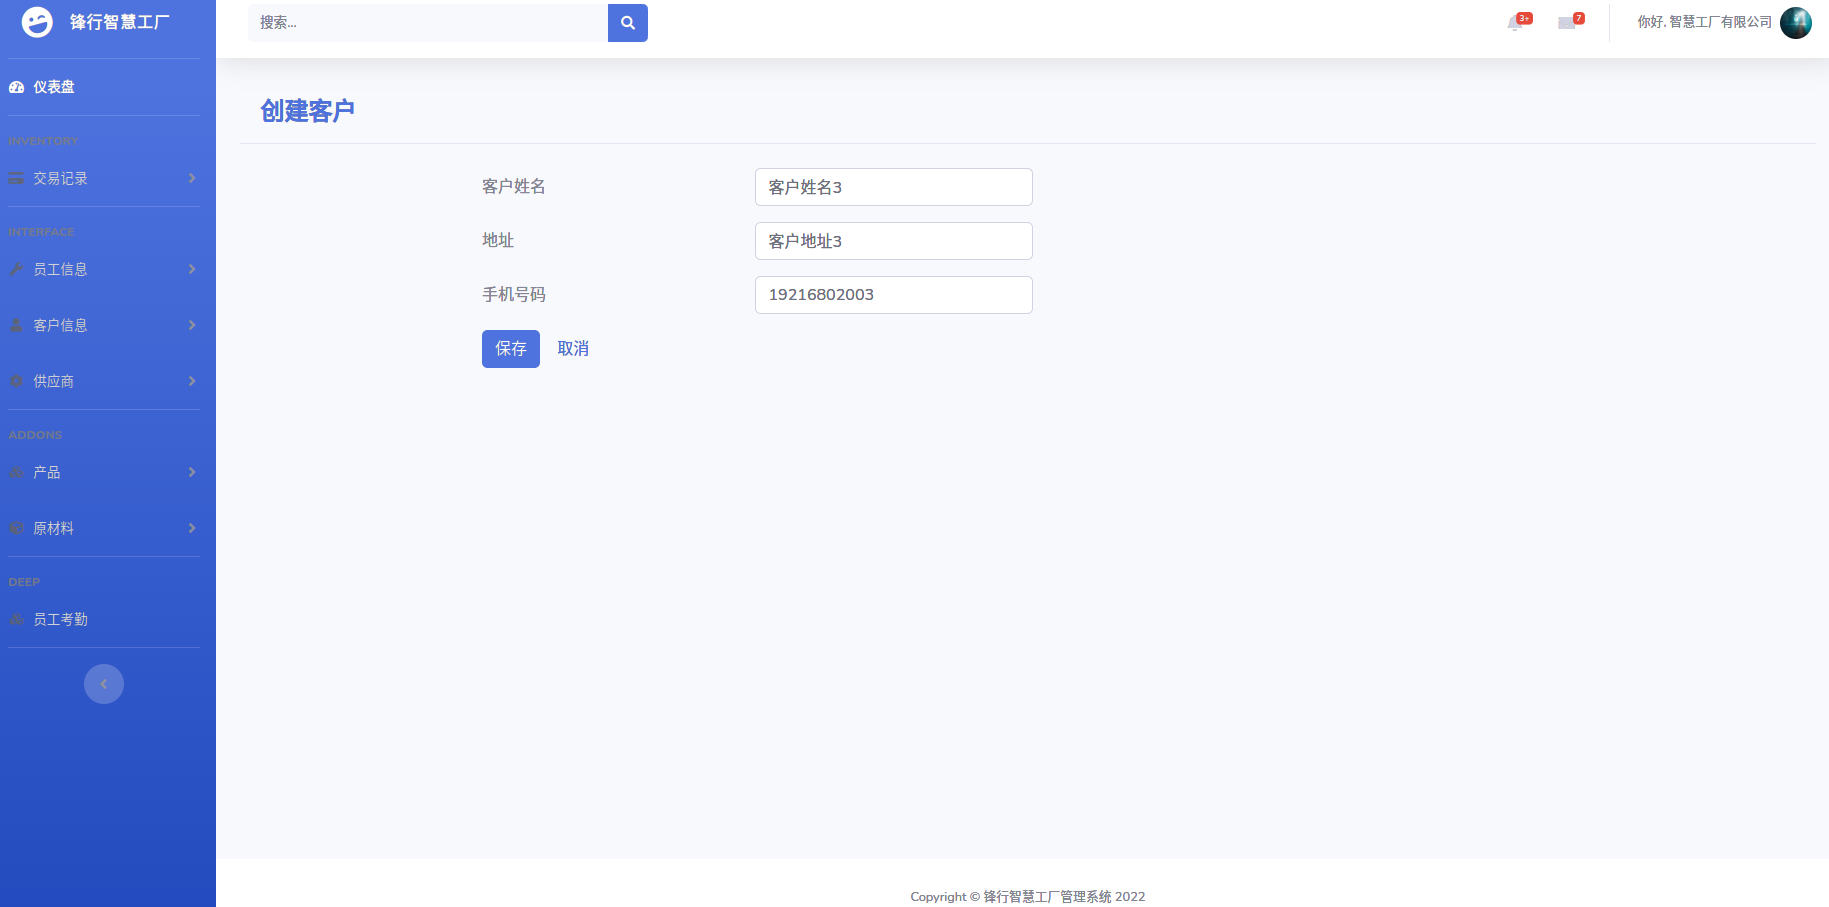
\includegraphics[width=\textwidth]{figures/6addnewcustomer.png}
        % \subcaption{添加客户测试图}
        % \label{fig:adnucstm}
    \end{subfigure}
    % \\
    % \begin{subfigure}{.35\textwidth}
    %     \centering
    %     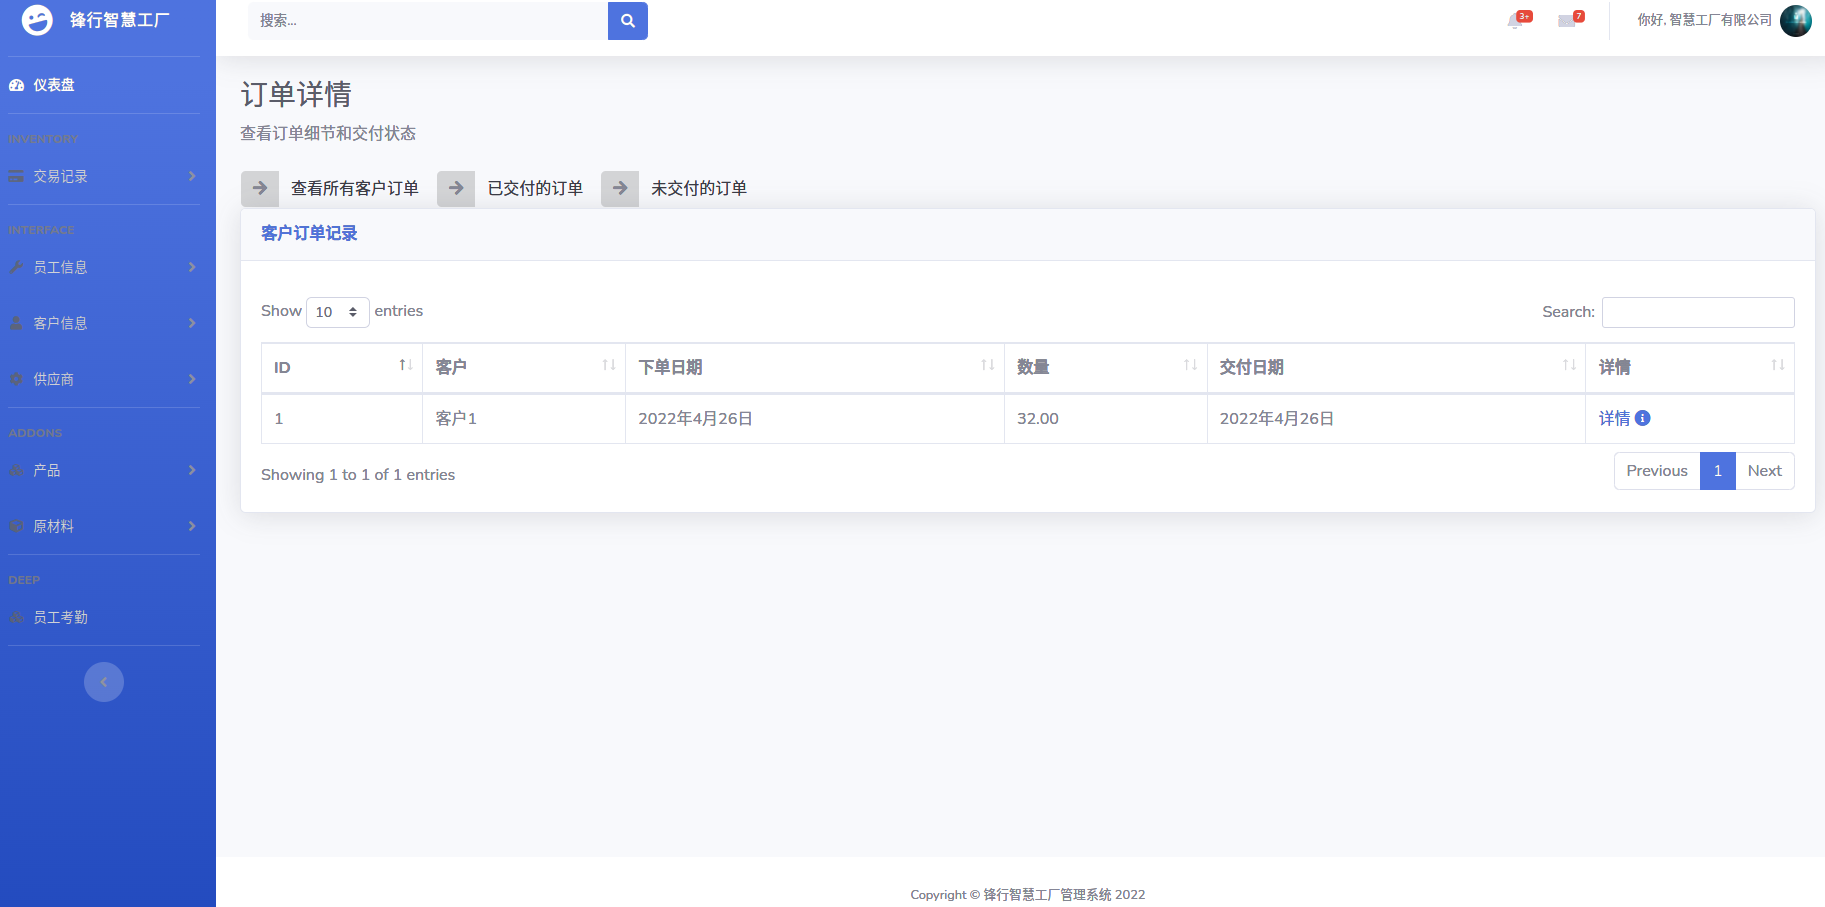
\includegraphics[width=\textwidth]{figures/6viewallorders.png}
    %     % \subcaption{查看所有客户订单测试图}
    %     % \label{fig:vuaods}
    % \end{subfigure}
    % \qquad
    % \begin{subfigure}{.35\textwidth}
    %     \centering
    %     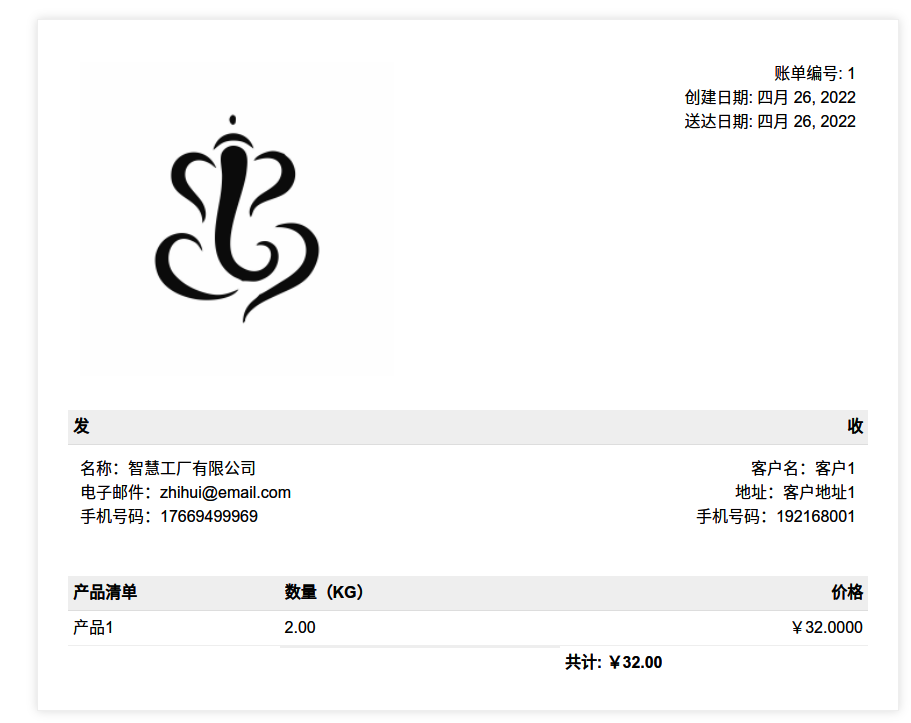
\includegraphics[width=\textwidth]{figures/6orderdetails.png}
    %     % \subcaption{查看订单收据测试图}
    %     % \label{fig:vuoddtls}
    % \end{subfigure}
    \caption{客户信息管理测试图}
    \label{fig:cstmtst}
\end{figure}

同理,可对供应商信息、产品信息以及原材料信息进行查看与添加功能测试,如图\ref{fig:otstst}所示。查看所有供应商信息、为添加供应商功能测试。

\begin{figure}[H]
    % \centering
    % \begin{subfigure}{.35\textwidth}
        \centering
        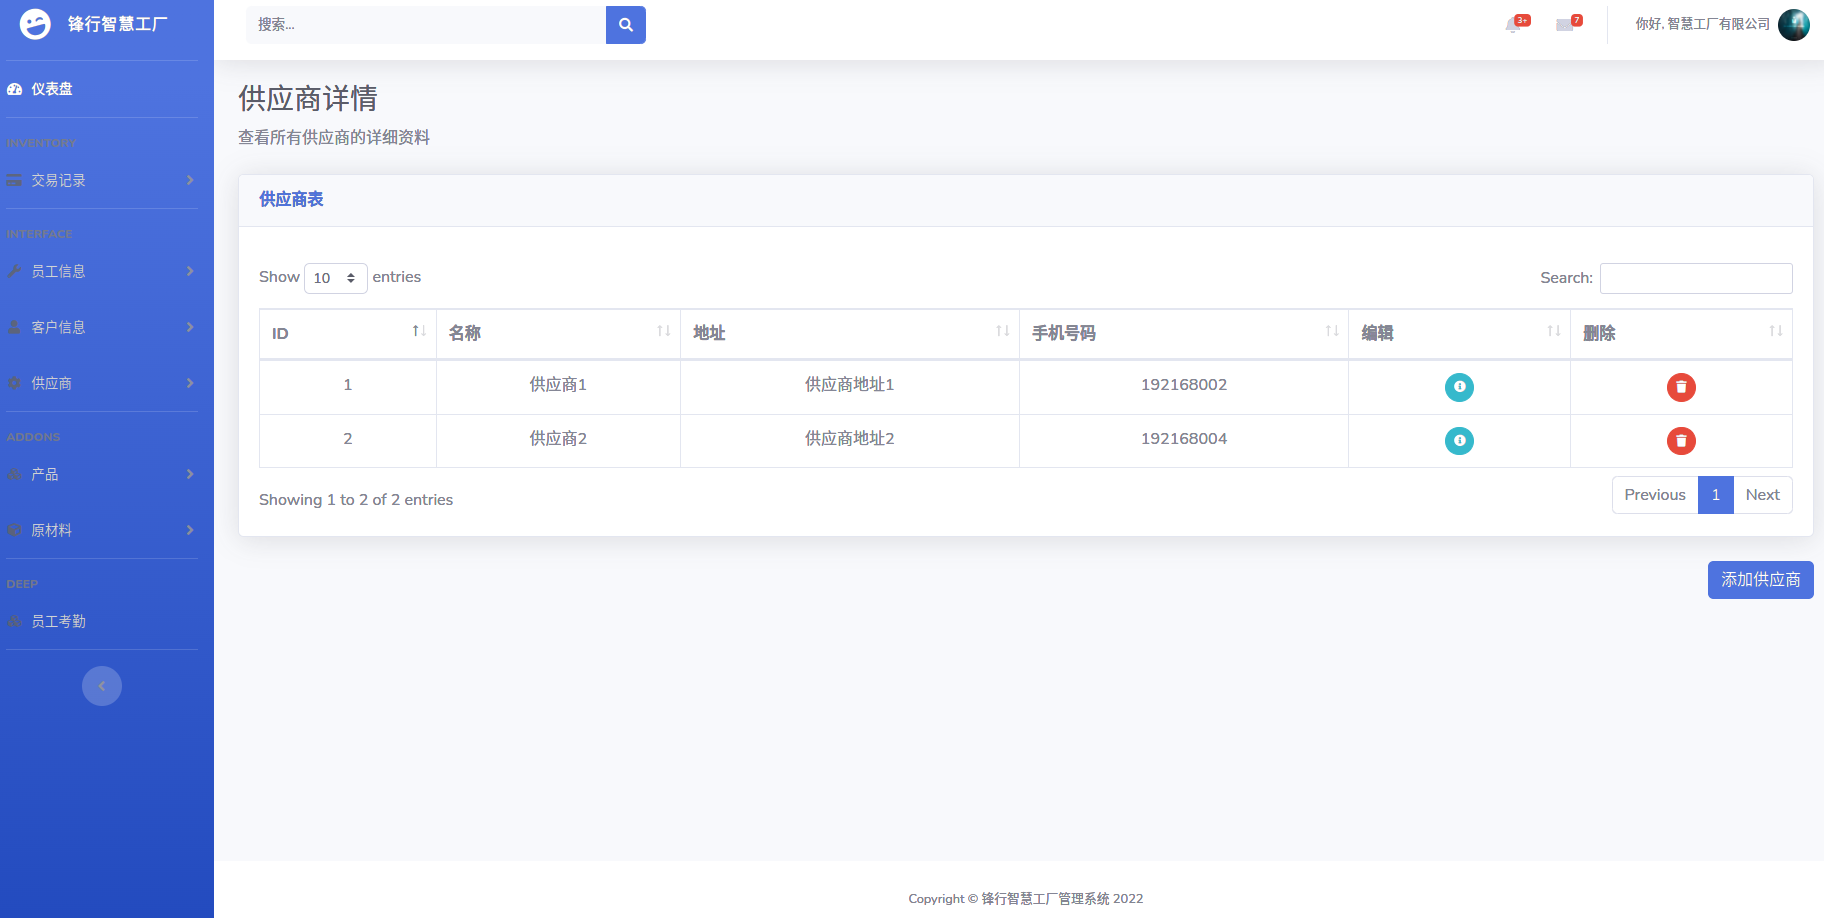
\includegraphics[width=.75\textwidth]{figures/6viewallsupplier.png}
        % \subcaption{查看供应商信息详情图}
        % \label{fig:vuaspie}
    % \end{subfigure}
    % \qquad
    % \begin{subfigure}{.35\textwidth}
    %     \centering
    %     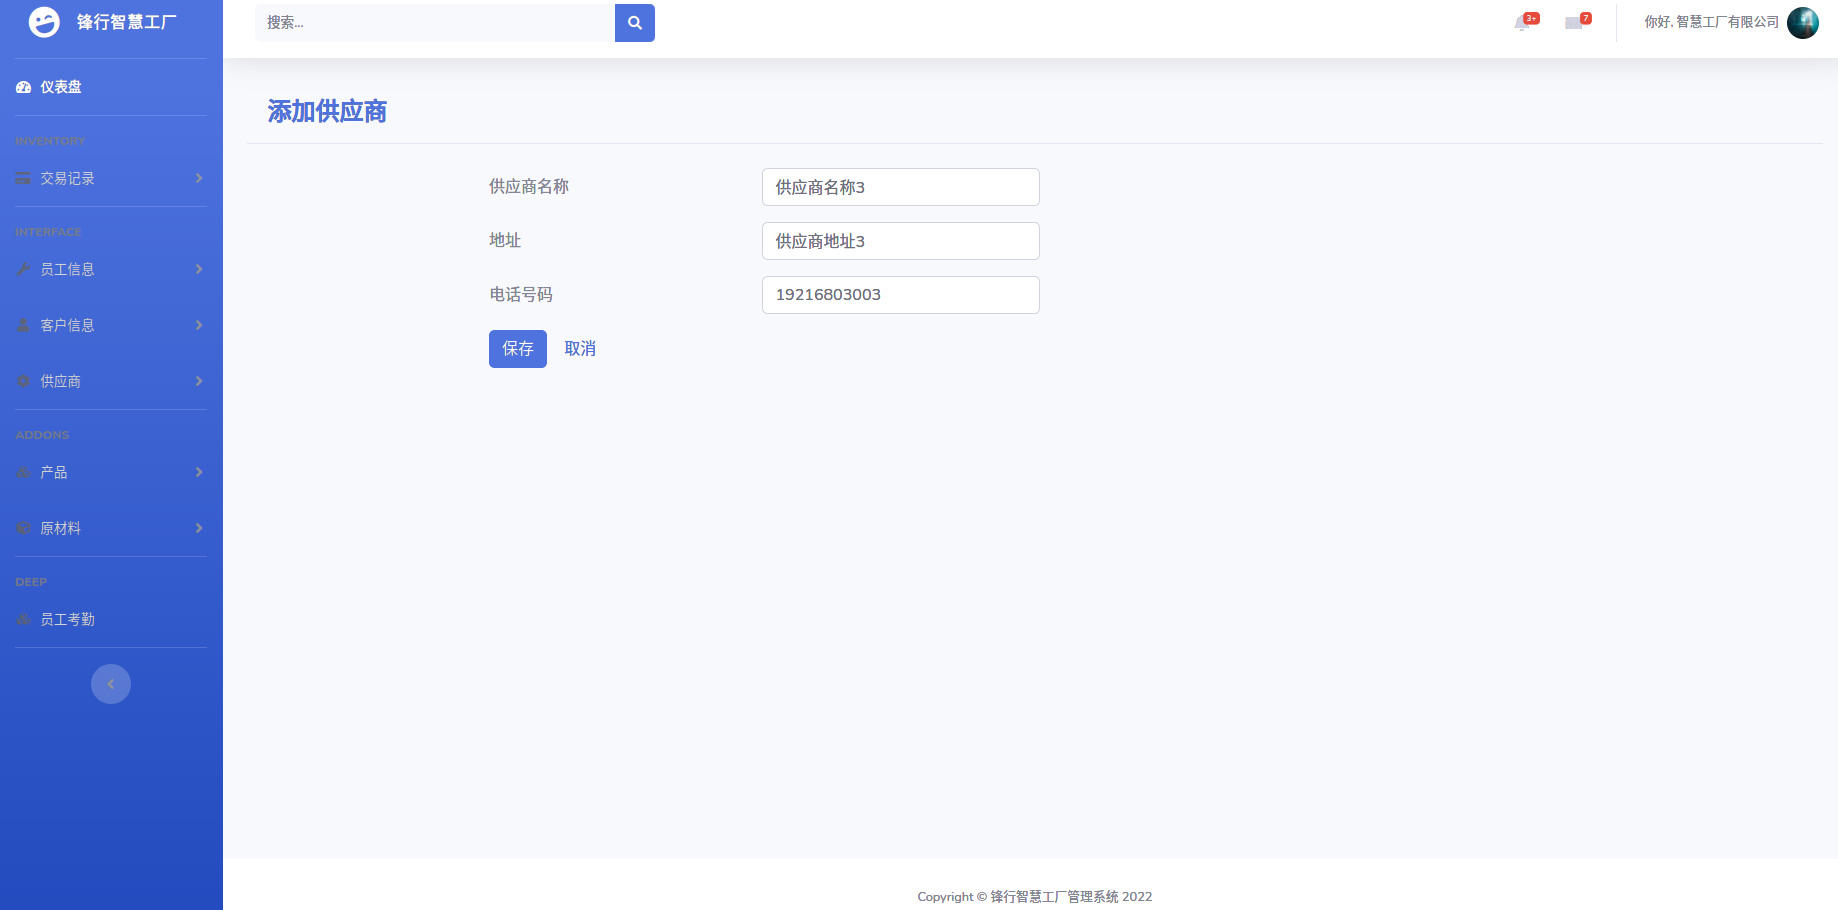
\includegraphics[width=\textwidth]{figures/6addnewsupplier.png}
    %     % \subcaption{添加供应商测试图}
    %     % \label{fig:adspie}
    % \end{subfigure}
    % \\
    % \begin{subfigure}{.35\textwidth}
    %     \centering
    %     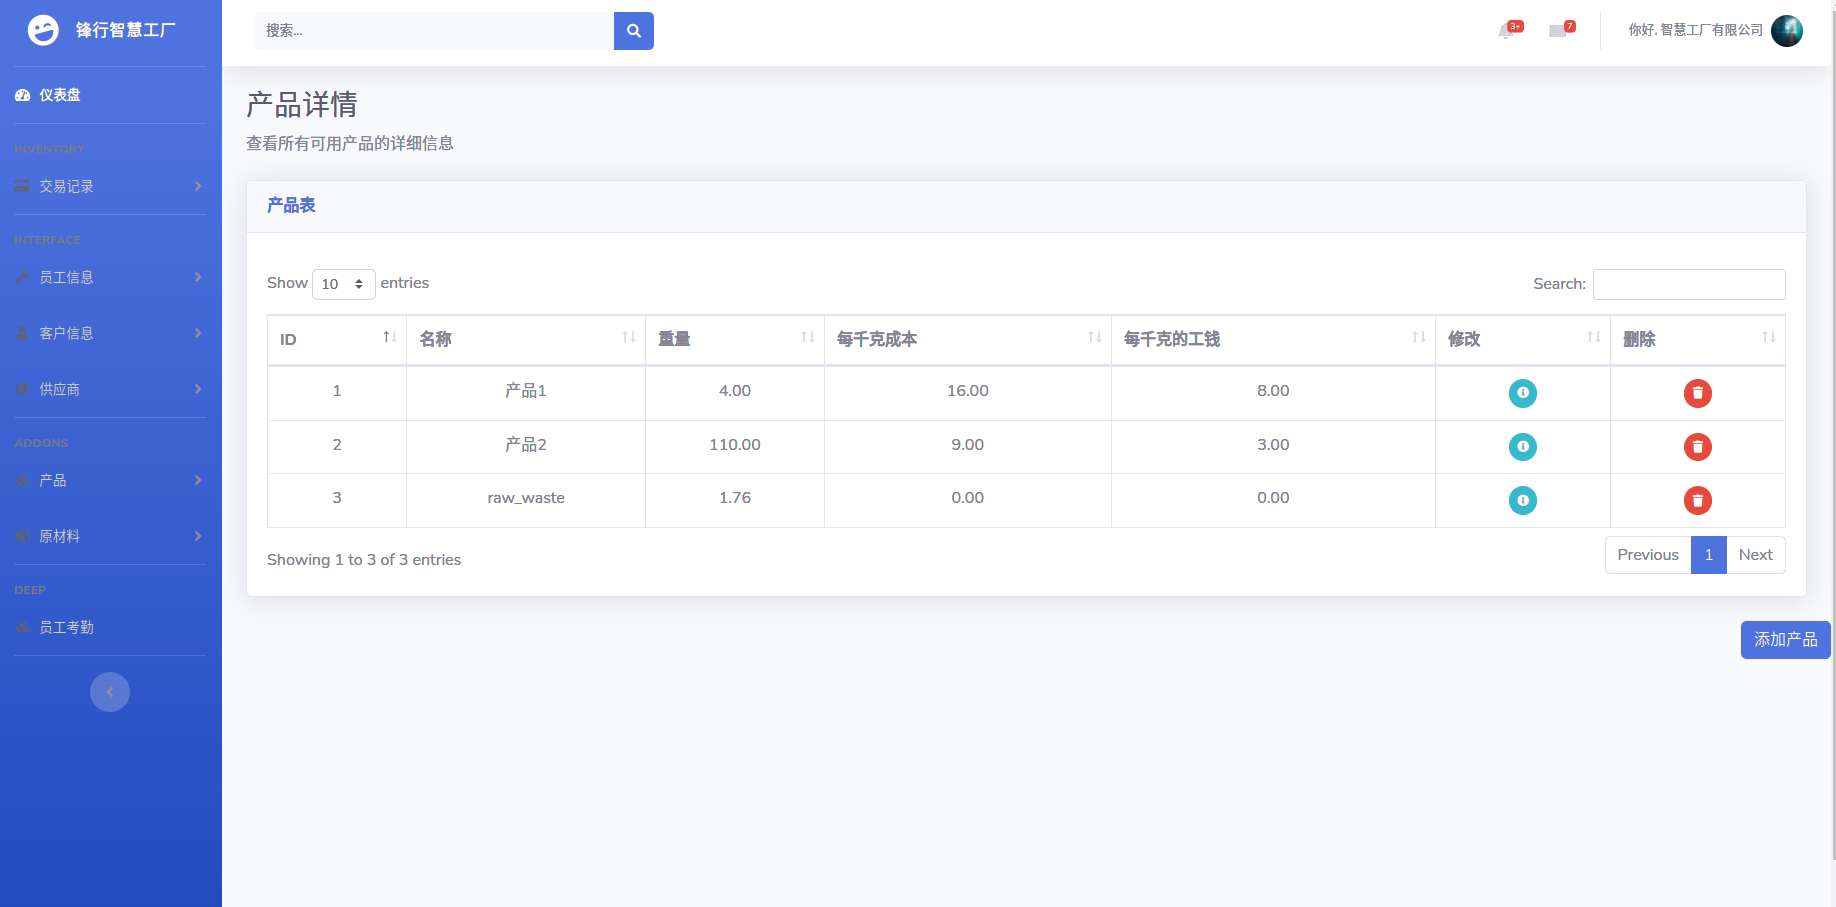
\includegraphics[width=\textwidth]{figures/6viewallproduct.png}
    %     % \subcaption{查看所有产品详情测试图}
    %     % \label{fig:vuaprdct}
    % \end{subfigure}
    % \qquad
    % \begin{subfigure}{.35\textwidth}
    %     \centering
    %     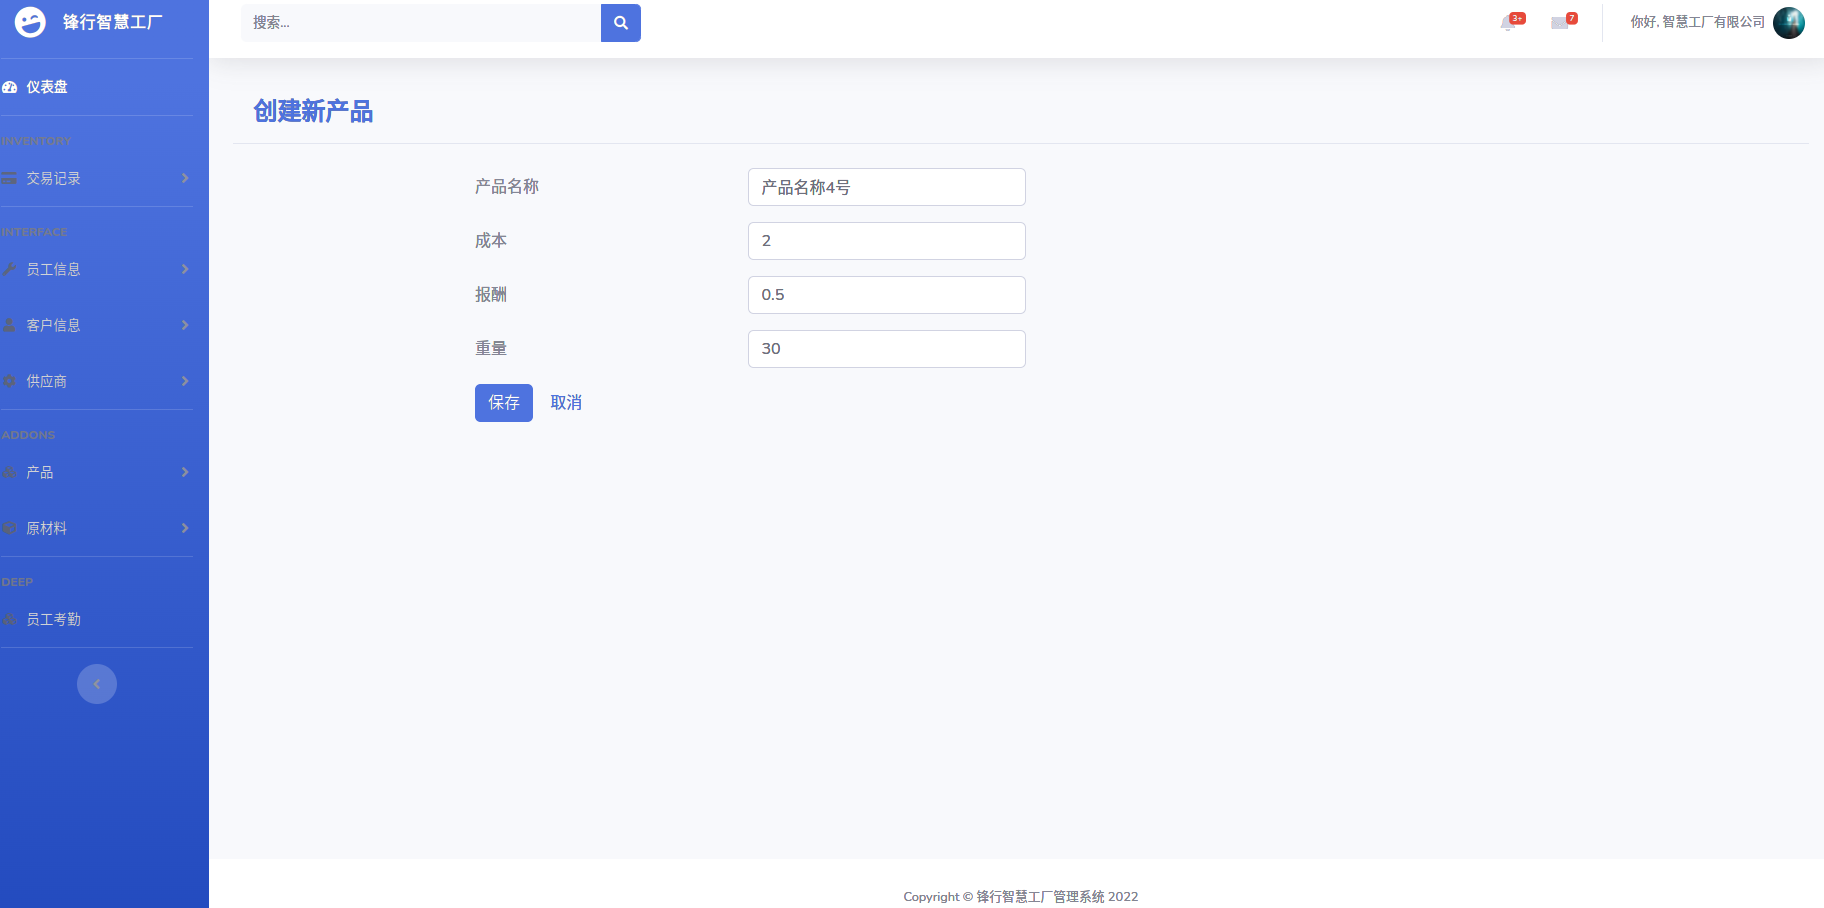
\includegraphics[width=\textwidth]{figures/6addnewproduct.png}
    %     % \subcaption{添加新产品功能测试图}
    %     % \label{fig:adnuprdct}
    % \end{subfigure}
    % \\
    % \begin{subfigure}{.35\textwidth}
    %     \centering
    %     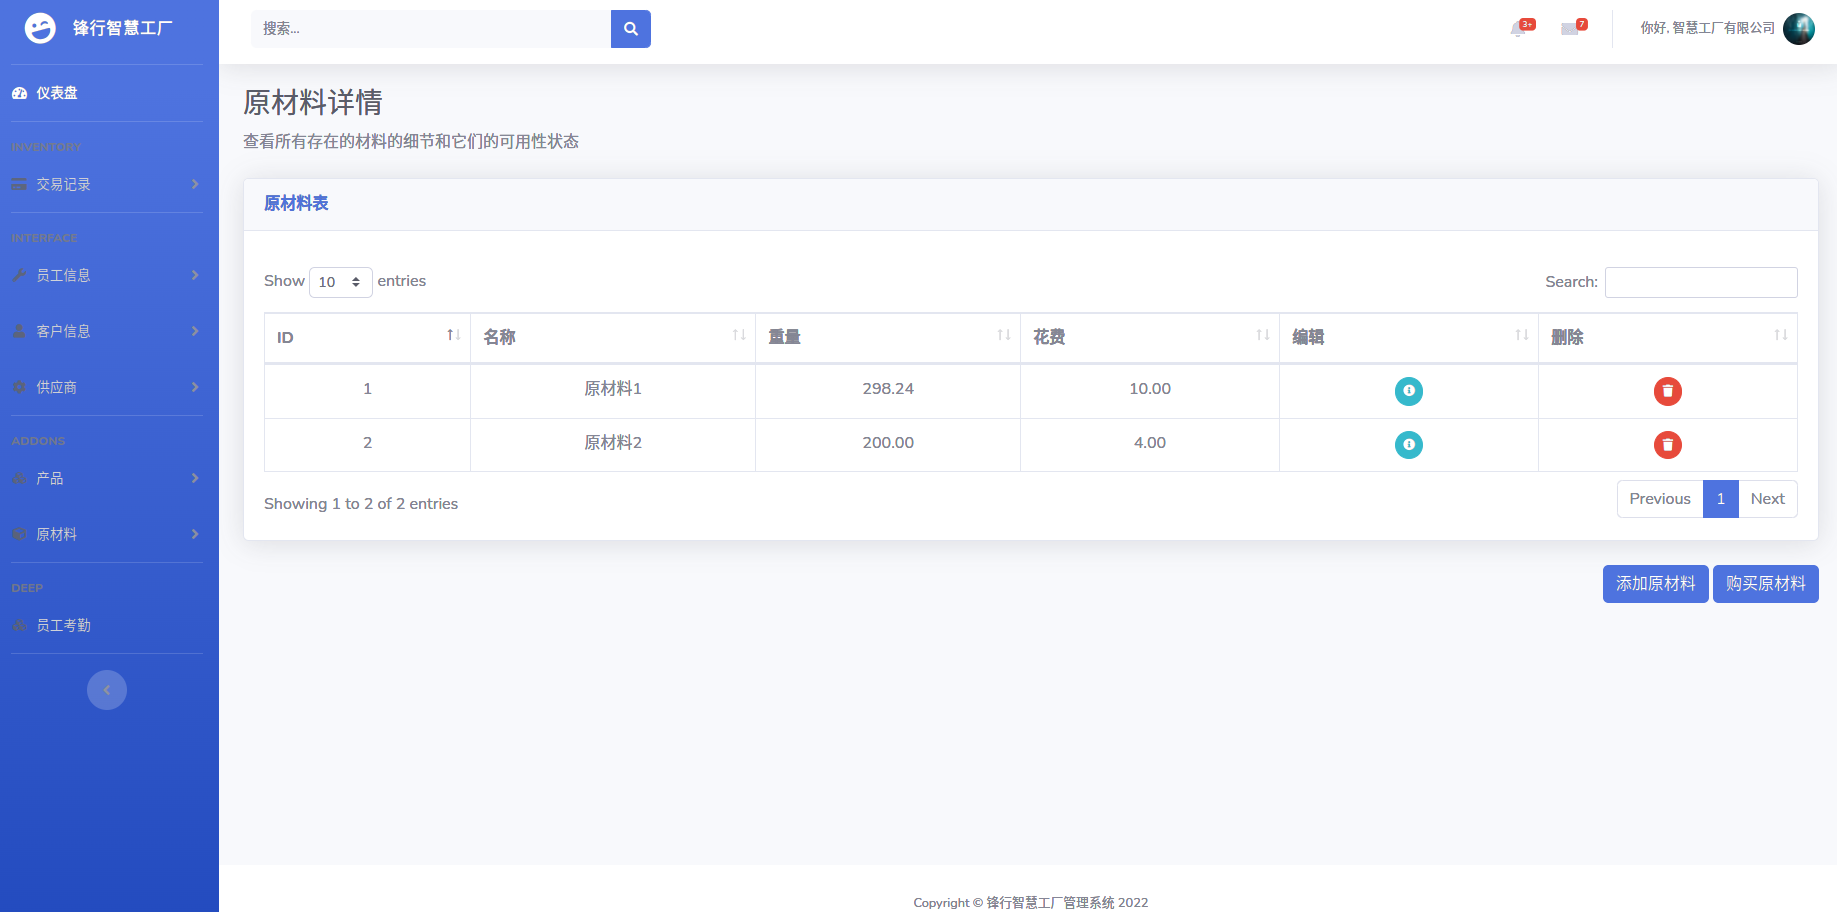
\includegraphics[width=\textwidth]{figures/6viewallmaterial.png}
    %     % \subcaption{查看所有原材料详情测试图}
    %     % \label{fig:vuamtra}
    % \end{subfigure}
    % \qquad
    % \begin{subfigure}{.35\textwidth}
    %     \centering
    %     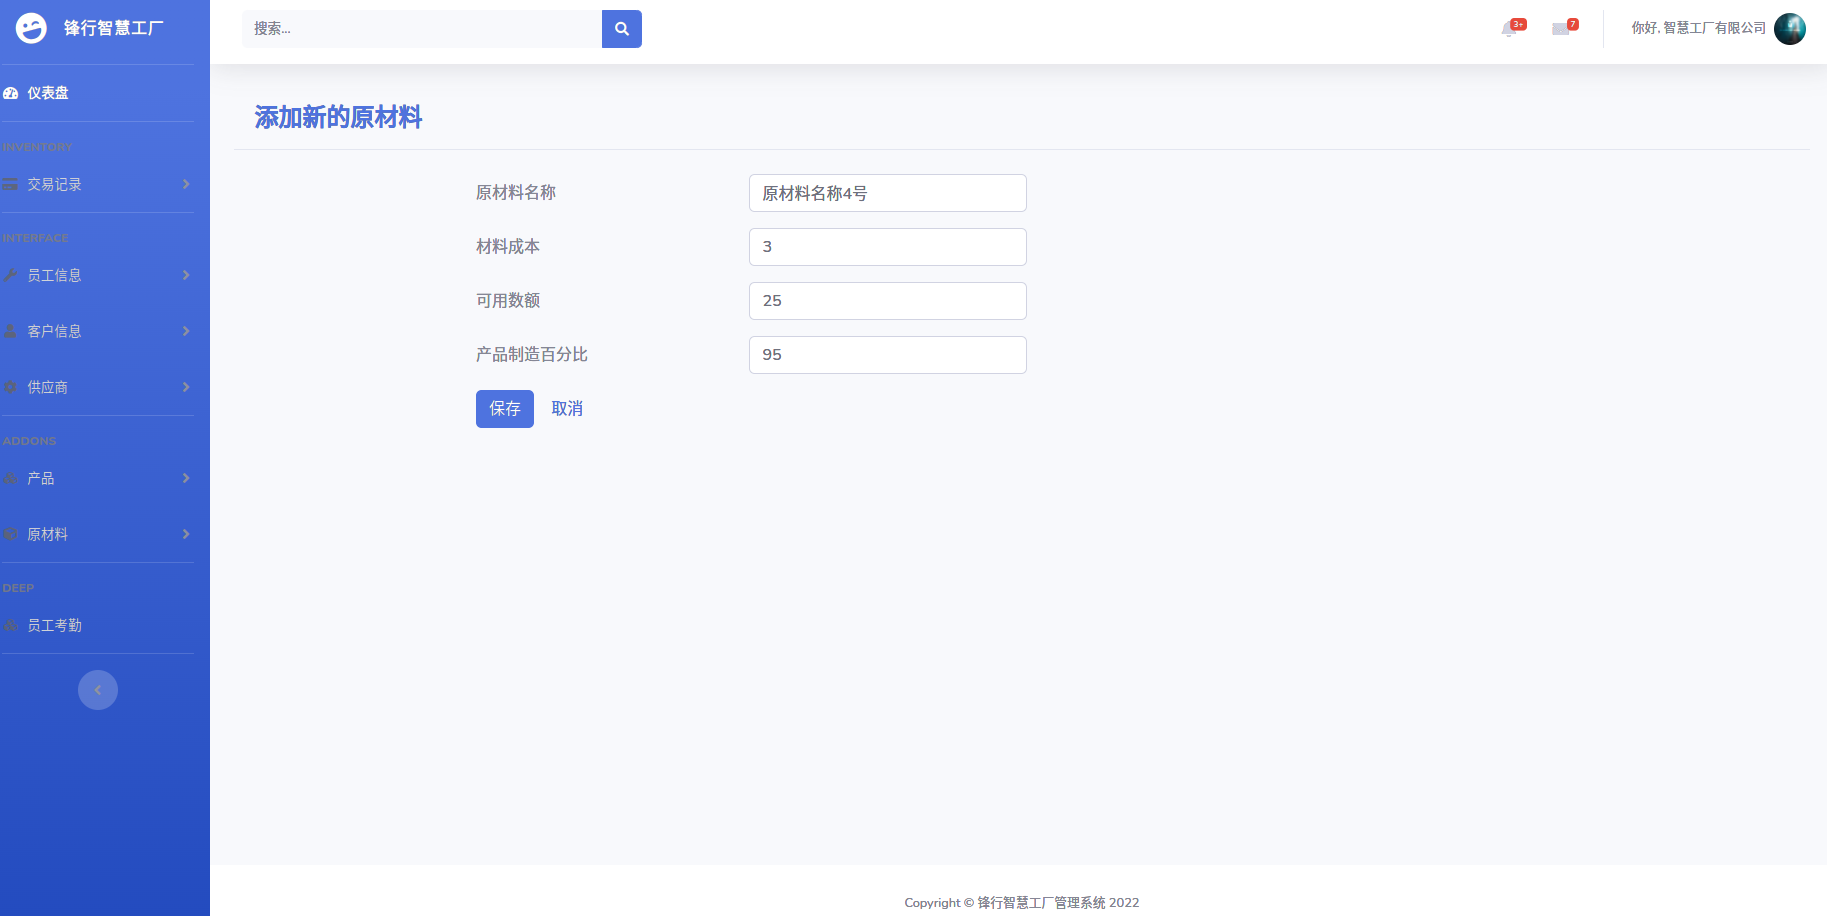
\includegraphics[width=\textwidth]{figures/6addnewmaterial.png}
    %     % \subcaption{添加新原材料类型测试图}
    %     % \label{fig:adnumtra}
    % \end{subfigure}
    \caption{供应商功能测试图}
    \label{fig:otstst}
\end{figure}

\subsection{员工考勤功能测试}

管理员进入员工考勤页面,首先查询当前的签到表记录并且将签到记录表展示在后台页面上,如图\ref{fig:empleatdc}所示。

\begin{figure}[H]
    \centering
    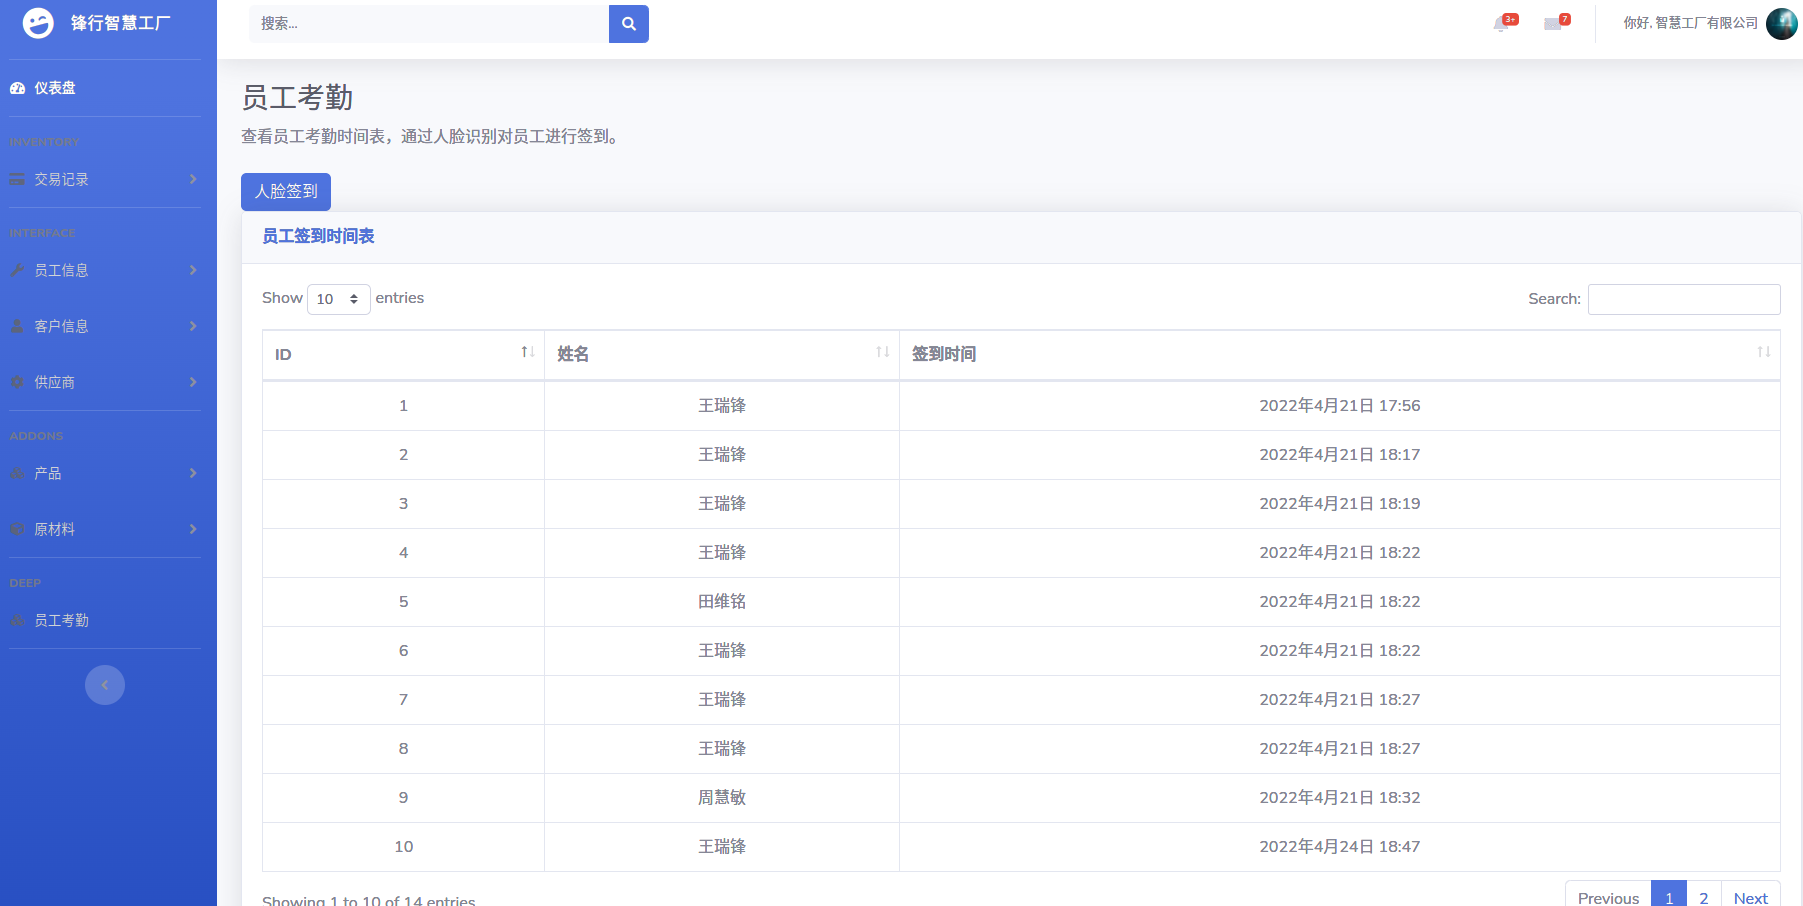
\includegraphics[width=.55\textwidth]{figures/6employeeattendance.png}
    \caption{员工考勤签到记录页面图}
    \label{fig:empleatdc}
\end{figure}

表\ref{tab:fcrcgnts}为员工考勤功能中人脸识别的测试用例表。

\begin{table}[H]
    \zihao{5}
    \centering
    \caption{人脸识别签到功能用例表}
    \label{tab:fcrcgnts}
    \begin{tabularx}{.95\textwidth}{p{2em}<{\centering}X<{\centering}p{16em}<{\centering}X<{\centering}X<{\centering}}
        \toprule
        序号 & 操作 & 输入及说明 & 期望结果 & 实际结果 \\
        \midrule
        1 & 人脸签到 & 根据系统提示拍摄员工人脸图像 & 签到成功 & 预期结果 \\
        2 & 人脸签到 & 员工佩戴口罩进行人脸识别签到 & 签到成功 & 预期结果 \\
        3 & 人脸签到 & 非员工人员进行人脸识别 & 签到失败 & 预期结果 \\
        4 & 人脸签到 & 人脸识别过程中键入退出字符 & 识别退出 & 预期结果 \\
        \bottomrule
    \end{tabularx}
\end{table}

当点击人脸签到按钮时,首先调用摄像头对当前场景进行拍摄,并且将图像输入至人脸识别模块对人脸进行检测识别,如果在第一帧的时刻就已经识别出哪位员工在进行人脸签到,就直接向签到记录表中插入一条新签到记录,若人脸识别模块没有认出员工人脸图像,便打开一个摄像头窗口以便于人脸图像位置、姿势以及光照等调节,如图\ref{fig:fcrcgnttst}所示。左图为第一帧未能识别人脸图像之后弹出的摄像窗口以便于调整姿势、角度和光照等环境调节,右图为佩戴口罩之后进行人脸识别签到测试。经过反复测试,该系统有着较高的准确率与较快的识别速度,可以应对日常工厂管理员工考勤场景。

\begin{figure}[H]
    \centering
    \begin{subfigure}{.45\textwidth}
        \centering
        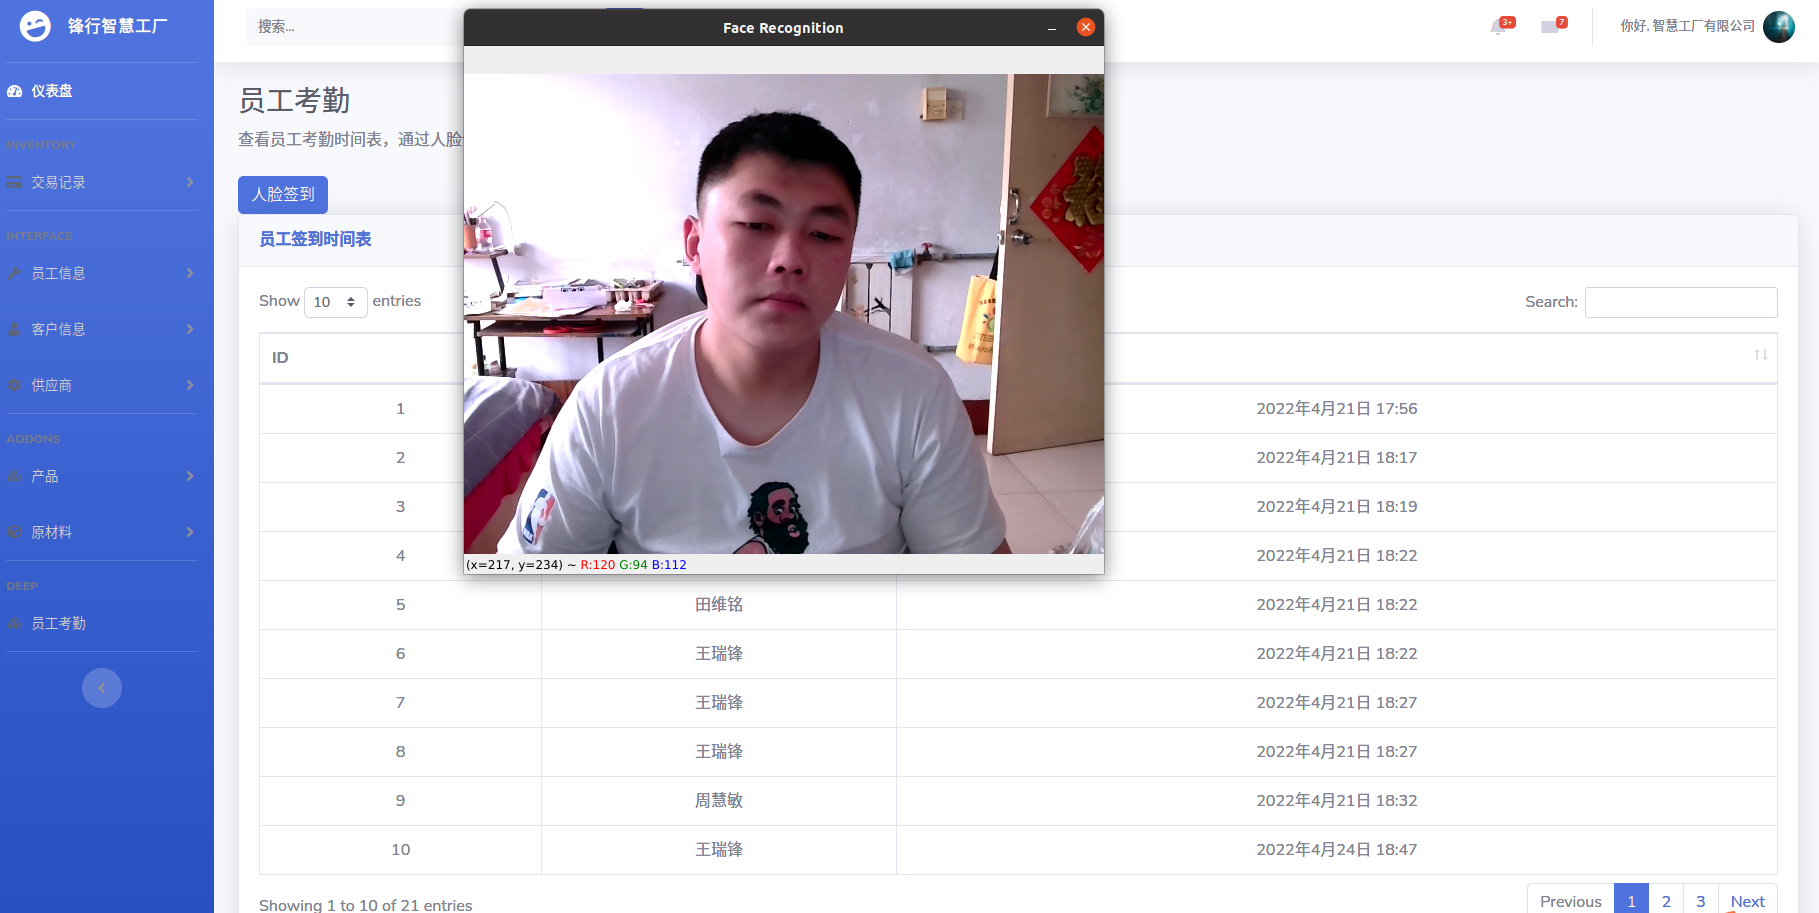
\includegraphics[width=\textwidth]{figures/6facerecerror.png}
        % \subcaption{弹出摄像图像窗口图}
        % \label{fig:fcrcgnt}
    \end{subfigure}
    \qquad
    \begin{subfigure}{.45\textwidth}
        \centering
        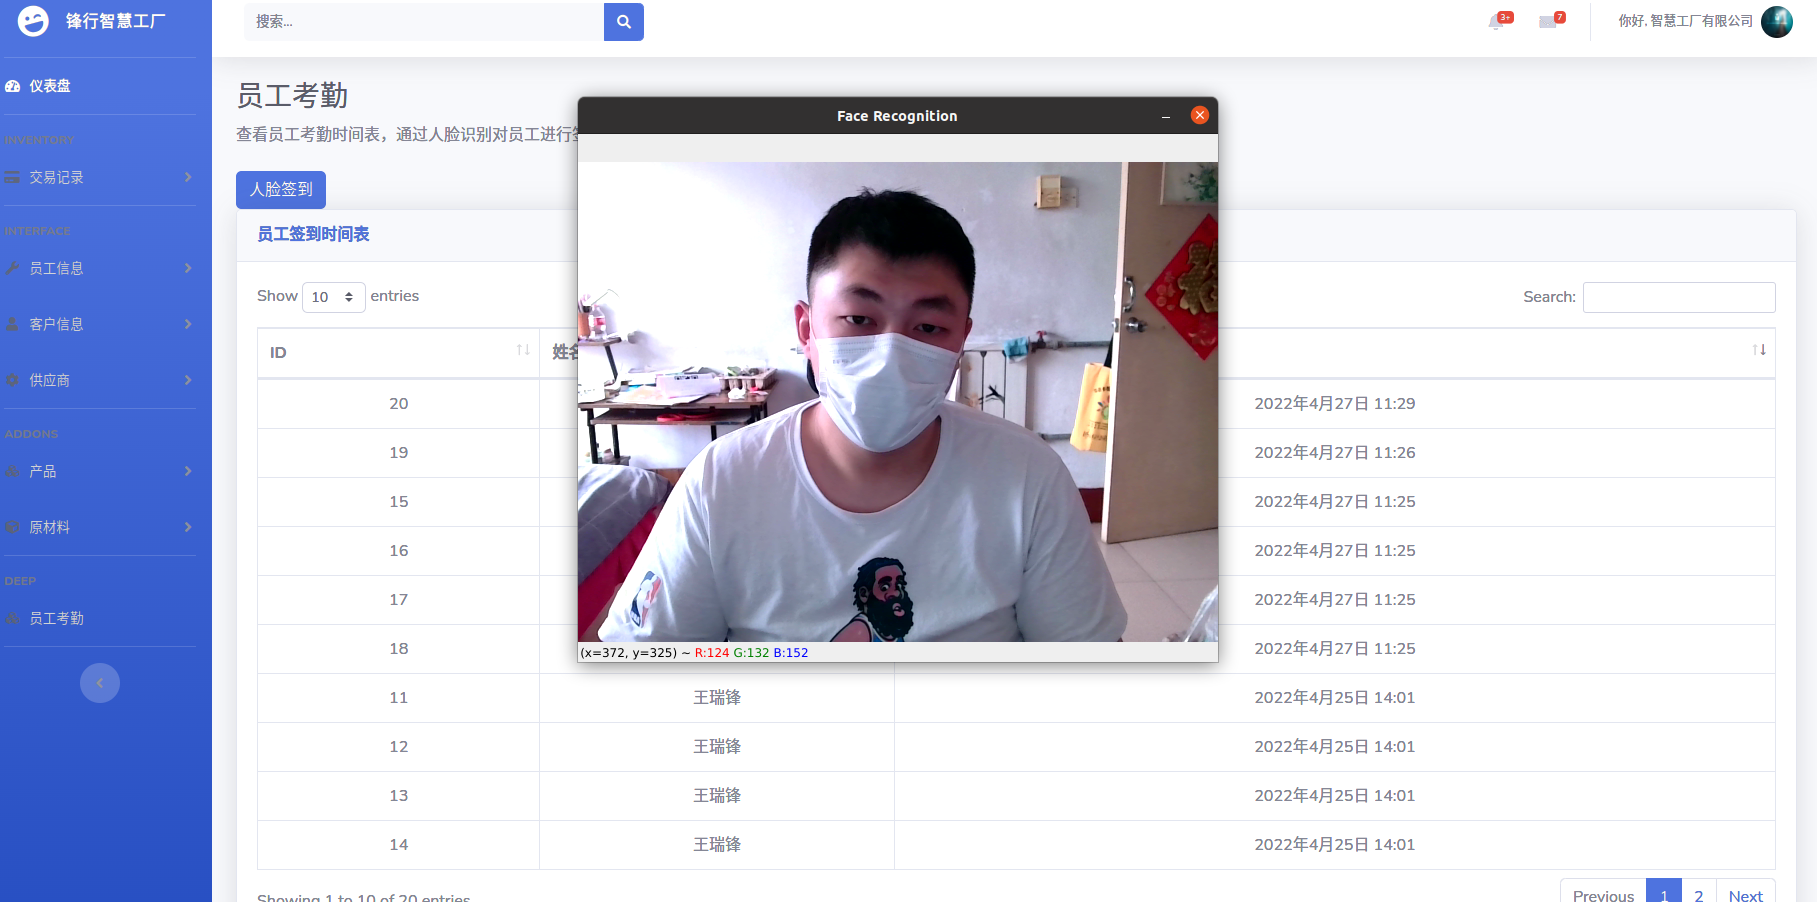
\includegraphics[width=\textwidth]{figures/6maskedfacerec.png}
        % \subcaption{佩戴口罩人脸识别测试图}
        % \label{fig:mskdfcrcgnt}
    \end{subfigure}
    \caption{人脸识别签到功能测试图}
    \label{fig:fcrcgnttst}
\end{figure}